\section{Hai mặt phẳng song song}
\subsection{Lý thuyết}
\subsubsection{Hai mặt phẳng song song}
Hai mặt phẳng được gọi là song song nếu chúng không có điểm chung. Kí hiệu: $\left( \alpha  \right)\parallel \left( \beta  \right)hay\left( \beta  \right)\parallel \left( \alpha  \right)$\\
Khi đó: $\left( \alpha  \right)\parallel \left( \beta  \right)\Leftrightarrow \left( \alpha  \right)\cap \left( \beta  \right)=\varnothing $\\
Chú ý: Nếu $\left( \alpha  \right)\parallel \left( \beta  \right)$ thì mọi đường thẳng $a\subset \left( \alpha  \right)$ đều song song với $\left( \beta  \right)$.
\begin{center}
	\begin{tikzpicture}
		\tkzDefPoints{0/0/A, 4/0/B, 1.5/1.5/D, 0/-2/A'}
		\coordinate (C) at ($(D)+(B)-(A)$);
		\coordinate (B') at ($(B)+(A')-(A)$);
		\coordinate (C') at ($(C)+(A')-(A)$);
		\coordinate (D') at ($(D)+(A')-(A)$);
		\coordinate (E) at ($(C)!0.8!(D)$);
		\coordinate (F) at ($(A)!0.8!(B)$);
		\coordinate (M) at ($(A)!0.7!(E)$);
		\coordinate (N) at ($(C)!0.7!(F)$);
		\tkzDrawSegment(M,N)
		\tkzDrawPolygon(A,B,C,D)
		\tkzDrawPolygon(A',B',C',D')     
		\tkzMarkAngle[size=.7](B,A,D)
		\tkzMarkAngle[size=.7](B',A',D')
		\draw (A) node[xshift=12pt,yshift=5pt]{$\alpha$};
		\draw (A') node[xshift=12pt,yshift=5pt]{$\beta$};   
		\draw ($(M)!0.5!(N)$) node[above]{$d$};
	\end{tikzpicture}
\end{center}
\subsubsection{Điều kiện và tính chất của hai mặt phẳng song song}
\begin{tc}
	Nếu mặt phẳng $\left( \alpha  \right)$ chứa hai đường thẳng cắt nhau và hai đường thẳng này cùng song song với mặt phẳng $\left( \beta  \right)$ thì $\left( \alpha  \right)$ song song với $\left( \beta  \right)$.
\end{tc}
\begin{tc}
	Qua một điểm nằm ngoài mặt phẳng có một và chỉ một mặt phẳng song song với mặt phẳng đã cho.
\end{tc}
\begin{tc}
	Nếu đường thẳng $d$ song song với mặt phẳng$\left( P \right)$thì có duy nhất một mặt phẳng $\left( Q \right)$chứa $d$ và song song với $\left( P \right)$.
\end{tc}
\begin{tc}
	Hai mặt phẳng phân biệt cùng song song với mặt phẳng thứ ba thì song song với nhau.
\end{tc}
\begin{tc}
	Cho điểm $A\notin \left( P \right)$. khi đó mọi đthẳng đi qua $A$ và song song với $\left( P \right)$đều nằm trong một mặt phẳng $\left( Q \right)$ đi qua $A$ và song song với $\left( P \right)$.
\end{tc}
\begin{tc}
	Nếu một mặt phẳng cắt một trong hai mặt phẳng song song thì cũng cắt mặt phẳng kia và các giao tuyến của chúng song song với nhau.
\end{tc}
\begin{hq}
	Hai mặt phẳng song song chắn trên hai cát tuyến song song những đoạn thẳng bằng nhau.
\end{hq}
\subsubsection{Định lý Thalès}
\begin{dl}
	Ba mặt phẳng đôi một song song chắn trên hai cát tuyến bất kì những đoạn thẳng tương ứng tỉ lệ.
\end{dl}
\begin{center}
	\begin{tikzpicture}[font=\footnotesize]
		\coordinate (A) at (0,0);
		\coordinate (B) at (4.2,0);
		\coordinate (C) at (5,1.2);
		\coordinate (A1) at (0.3,2);
		\coordinate (M) at (1.8,6);
		\coordinate (Q) at (2.3,6);
		\coordinate (N) at (1,-0.5);
		\coordinate (P) at (4,-0.5);
		\coordinate (D) at ($(C)-(B)+(A)$);
		\coordinate (B1) at ($0.85*(B)-0.85*(A)+(A1)$);
		\coordinate (C1) at ($0.95*(D)-0.95*(A)+(B1)$);
		\coordinate (D1) at ($(A1)-(B1)+(C1)$);
		\coordinate (X) at ($(M)!0.83!(N)$);
		\coordinate (Y) at ($(M)!0.55!(N)$);
		\coordinate (Z) at ($(M)!0.23!(N)$);
		\coordinate (X1) at ($(Q)!0.85!(P)$);
		\coordinate (Y1) at ($(Q)!0.5!(P)$);
		\coordinate (Z1) at ($(Q)!0.2!(P)$);
		\foreach \x in {A,B,C,D}
		\coordinate (\x2) at ($(\x)!2!(\x1)$); 
		\path[name path=mn] (M)--(N); 
		\path[name path=pq] (P)--(Q);
		\path[name path=ab] (A)--(B); 
		\path[name path=a1b1] (A1)--(B1);
		\path[name path=a2b2] (A2)--(B2);
		\path[name intersections={of=mn and ab,by=E}];
		\path[name intersections={of=mn and a1b1,by=F}];
		\path[name intersections={of=mn and a2b2,by=G}];
		\path[name intersections={of=pq and ab,by=E1}];
		\path[name intersections={of=pq and a1b1,by=F1}];
		\path[name intersections={of=pq and a2b2,by=G1}];
		\draw (A)--(B)--(C)--(D)--cycle (A1)--(B1)--(C1)--(D1)--cycle (A2)--(B2)--(C2)--(D2)--cycle (N)--(E) (E1)--(P) (F)--(X)node[left]{$C$}--(X1)node[right]{$C'$}--(F1) (G)--(Y)node[left]{$B$}--(Y1)node[right]{$B'$}--(G1) (M)node[left]{$d$}--(Z)node[left]{$A$}--(Z1)node[right]{$A'$}--(Q)node[right]{$d'$};
		\draw[dashed] (E)--(X) (E1)--(X1) (F)--(Y) (F1)--(Y1) (G)--(Z) (G1)--(Z1);
		\draw pic[draw,"$R$"]{angle=B--A--D} pic[draw,"$Q$"]{angle=B1--A1--D1} pic[draw,"$P$"]{angle=B2--A2--D2};
	\end{tikzpicture}
\end{center}
\subsubsection{Hình lăng trụ}
\begin{dn}
	Trên mặt phẳng $\left( \alpha  \right)$ cho đa giác ${{A}_{1}}{{A}_{2}}...{{A}_{n}}$, từ các đỉnh của đa giác dựng các đường thẳng song song cắt mặt phẳng $\left( \alpha ' \right)$ song song với $\left( \alpha  \right)$ tại các điểm ${{A}_{1}}',{{A}_{2}}',..,{{A}_{n}}'$. Hình hợp bởi hai miền đa giác ${{A}_{1}}{{A}_{2}}...{{A}_{n}}$ và ${{A}_{1}}'{{A}_{2}}'...{{A}_{n}}'$với các hình chữ nhật ${{A}_{1}}{{A}_{2}}{{A}_{2}}'{{A}_{1}}'$, ${{A}_{2}}{{A}_{3}}{{A}_{3}}'{{A}_{2}}'$,. được gọi là hình lăng trụ.
\end{dn}
\begin{center}
	\begin{tikzpicture}[font=\footnotesize]
		\coordinate (A) at (0,0);
		\coordinate (B) at (5.5,0);
		\coordinate (C) at (6.5,2);
		\coordinate (A1) at (0,4.5);
		\coordinate (M1) at (1,7);
		\coordinate (N1) at (2,-1);
		\coordinate (D) at ($(C)-(B)+(A)$);
		\coordinate (B1) at ($(B)-(A)+(A1)$);
		\coordinate (C1) at ($(C)-(B)+(B1)$);
		\coordinate (D1) at ($(C1)-(B1)+(A1)$);
		\coordinate (A11) at ($(M1)!.78!(N1)$);
		\coordinate[shift={(1,-0.3)}] (M2) at (1,7);
		\coordinate[shift={(3,-0.2)}] (M3) at (1,7);
		\coordinate[shift={(3.5,0.5)}] (M4) at (1,7);
		\coordinate[shift={(1.5,0.7)}] (M5) at (1,7);
		\coordinate[shift={(1,-0.3)}] (N2) at (2,-1);
		\coordinate[shift={(3,-0.2)}] (N3) at (2,-1);
		\coordinate[shift={(3.5,0.5)}] (N4) at (2,-1);
		\coordinate[shift={(1.5,0.7)}] (N5) at (2,-1);
		\coordinate[shift={(1,-0.3)}] (B11) at ($(M1)!.78!(N1)$);
		\coordinate[shift={(3,-0.2)}] (C11) at ($(M1)!.78!(N1)$);
		\coordinate[shift={(3.5,0.5)}] (D11) at ($(M1)!.78!(N1)$);
		\coordinate[shift={(1.5,0.7)}] (E11) at ($(M1)!.78!(N1)$);
		\coordinate (A22) at ($(M1)!.22!(N1)$);
		\coordinate[shift={(1,-0.3)}] (B22) at ($(M1)!.22!(N1)$);
		\coordinate[shift={(3,-0.2)}] (C22) at ($(M1)!.22!(N1)$);
		\coordinate[shift={(3.5,0.5)}] (D22) at ($(M1)!.22!(N1)$);
		\coordinate[shift={(1.5,0.7)}] (E22) at ($(M1)!.22!(N1)$);
		\path[name path=k1] (M1)--(N1); 
		\path[name path=k2] (M2)--(N2);
		\path[name path=k3] (M3)--(N3);
		\path[name path=k4] (M4)--(N4);
		\path[name path=k5] (M5)--(N5);
		\path[name path=ab] (A)--(B); 
		\path[name path=cd] (C)--(D);
		\path[name path=a1b1] (A1)--(B1);
		\path[name intersections={of=k1 and ab,by=E1}];
		\path[name intersections={of=k2 and ab,by=E2}];
		\path[name intersections={of=k3 and ab,by=E3}];
		\path[name intersections={of=k4 and ab,by=E4}];
		\path[name intersections={of=k5 and ab,by=E5}];
		\path[name intersections={of=k1 and cd,by=F1}];
		\path[name intersections={of=k4 and cd,by=F4}];
		\path[name intersections={of=k1 and a1b1,by=G1}];
		\path[name intersections={of=k2 and a1b1,by=G2}];
		\path[name intersections={of=k3 and a1b1,by=G3}];
		\path[name intersections={of=k4 and a1b1,by=G4}];
		\path[name intersections={of=k5 and a1b1,by=G5}];
		\draw (M1)--(A22) (M2)--(B22) (M3)--(C22) (M4)--(D22) (M5)--(E22);
		\draw (F1)--(D)--(A)--(B)--(C)--(F4) (A1)--(B1)--(C1)--(D1)--cycle (A11)--(G1) (B11)--(G2) (C11)--(G3) (D11)--(G4) (E1)--(N1) (E2)--(N2) (E3)--(N3) (E4)--(N4) (E5)--(N5) (A11)--(B11)--(C11)--(D11) (A22)--(B22)--(C22)--(D22)--(E22)--cycle;
		\draw[dashed] (A11)--(E1) (B11)--(E2) (C11)--(E3) (D11)--(E4) (E11)--(E5) (F1)--(F4) (A22)--(G1) (B22)--(G2) (C22)--(G3) (D22)--(G4) (E22)--(E11) (A11)--(E11)--(D11);
		\draw (A11) node[left] {$A_1$} (A22) node[left] {$A_1'$} (B11) node[below left] {$A_2$} (C11) node[below left] {$A_3$} (D11) node[right] {$A_4$} (E11) node[above left] {$A_5$} (B22) node[below left] {$A_2'$} (C22) node[below left] {$A_3'$} (D22) node[right] {$A_4'$} (E22) node[above left] {$A_5'$};
		\draw pic[draw,"$\alpha$"]{angle=B--A--D} pic[draw,"$\alpha'$"]{angle=B1--A1--D1};
	\end{tikzpicture}
\end{center}
\begin{tc}
	\begin{itemize}
		\item Các hình bình hành được gọi là các mặt bên, hai miền đa giác gọi là hai mặt đáy của lăng trụ.
		\item Hai đáy của lăng trụ là hai đa giác bằng nhau và nằm trên hai mặt phẳng song song với nhau.
		\item Các đoạn thẳng ${{A}_{1}}{{A}_{1}}',{{A}_{2}}{{A}_{2}}',...$ được gọi là các cạnh bên. Các cạnh bên của lăng trụ song song và bằng nhau.
		\item Ta gọi lăng trụ theo tên của đa giác đáy, tức là nếu đáy là tam giác thì gọi là lăng trụ tam giác, nếu đáy là tứ giác thì gọi là lăng trụ tứ giác.
	\end{itemize}
\end{tc}
\subsubsection{Hình hộp}
\begin{dn}
	Hình lăng trụ tứ giác có đáy là hình bình hành được gọi là hình hộp.
\end{dn}
\begin{center}
	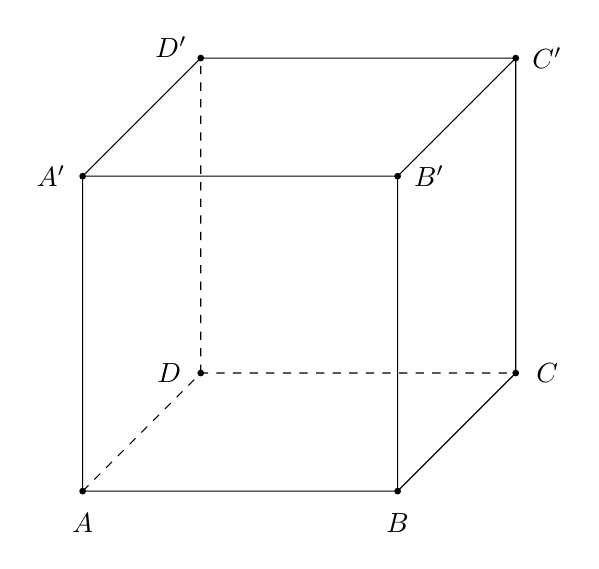
\begin{tikzpicture}
		\def\a{4} 
		\path
		(0,0) coordinate (A) 
		(\a,0) coordinate (B) 
		(1.5,1.5) coordinate (D) 
		(D)+(\a,0) coordinate (C);
		\foreach \x in {A,B,C,D}
		\path (\x)+(0,\a) coordinate(\x');	
		\draw[dashed] (A)--(D)--(C) (D)--(D');
		\draw(A')--(B')--(C')--(D')--(A')--(A)--(B)--(C)--(C') (B)--(B');
		\foreach \p/\g in {A/-90,B/-90,C/0,D/180,A'/180,B'/0,C'/0,D'/160}\draw[fill=black] (\p) circle (1pt)node[shift={(\g:.4)}]{$\p$};
	\end{tikzpicture}
\end{center}
\begin{tc}
	\begin{itemize}
		\item Hình hộp có sáu mặt đều là những hình bình hành.
		\item Hai mặt song song với nhau gọi là hai mặt đối diện, hình hộp có ba cặp mặt đối diện.
		\item Hai đỉnh của hình hộp được gọi là hai đỉnh đối diện nếu chúng không cùng nằm trên một mặt nào.
		\item Các đoạn thẳng nối hai đỉnh đối diện được gọi là các đường chéo. Bốn đường chéo cắt nhau tại trung điểm của mỗi đường, điểm đó gọi là tâm của hình hộp.
		\item Hai cạnh gọi là đối nhau nếu chúng song song nhưng không cùng nằm trên một mặt của hình chóp.
		\item Mặt chéo của hình hộp là hình bình hành có hai cạnh là hai cạnh đối diện của hình hộp.
		\item Tổng bình phương các đường chéo của một hình hộp bằng tổng các bình phương của tất cả các cạnh của hình hộp đó.
	\end{itemize}
\end{tc}
\subsection{Hệ thống bài tập tự luận}
\begin{dang}{Chứng minh 2 mặt phẳng song song}		
	{\it Phương pháp:}
	\begin{enumerate} 
		\item $\heva{&\left( \alpha  \right)\supset a,b\\&a\cap b=I\\&a\parallel \left( \beta  \right), b\parallel \left( \beta  \right)\\}.\Rightarrow \left( \alpha  \right)\parallel \left( \beta  \right)$
		\item $\heva{&\left( \alpha  \right)\parallel \left( \gamma  \right)\\&\left( \beta  \right)\parallel \left( \gamma  \right)\\&\left( \alpha  \right)\ne \left( \beta  \right)\\}.\Rightarrow \left( \alpha  \right)\parallel \left( \beta  \right)$
	\end{enumerate}
\end{dang}
\subsubsection{Bài tập tự luận}
\begin{bt}%[1K4BC-2]
	Cho hình chóp $S.ABCD$ có đáy $ABCD$ là hình bình hành tâm $O$, gọi $M,N$ lần lượt là trung điểm của $SA,SD$. Chứng minh $\left( OMN \right)\parallel \left( SBC \right)$.
	
	\loigiai
	{ 
		\immini
		{
			Ta có $M,O$ lần lượt là trung điểm của $SA,AC$ nên $OM$ là đường trung bình của tam giác $SAC$ ứng với cạnh $SC$ do đó $OM\parallel SC$.\\
			Vậy $\heva{&OM\parallel SC\\&SC\subset \left( SBC \right).\\}\Rightarrow OM\parallel \left( SBC \right) \left( 1 \right)$.
		}
		{
			\begin{tikzpicture}[scale=1, font=\footnotesize, line join=round, line cap=round, >=stealth]
				\def \y{4}
				\def \z{3}	
				\coordinate (A) at (0,0);
				\coordinate (B) at ($(A)+(-2,-1)$);
				\coordinate (D) at ($(A)+(\y,0)$);
				\coordinate (C) at ($ (B)+(D)-(A) $);
				\coordinate (S) at ($ (A)+(0,\z) $);
				\path 
				($(S)!{1/2}!(A)$) coordinate (M)
				($(S)!{1/2}!(D)$) coordinate (N)
				($(A)!{1/2}!(C)$) coordinate (O)
				;	
				\draw [dashed] (B)--(A)--(D)--(B) (C)--(A)--(S) (O)--(M)--(N)--(O);
				\draw (S)--(B)--(C)--(D)--(S)--(C);
				\foreach \p/\g in {S/90,A/140,B/-90,C/-30,D/0,O/-90,M/180,N/30}\draw[fill=black] (\p) circle (1pt)node[shift={(\g:.3)}]{$\p$};
			\end{tikzpicture}
		}		
		Tương tự, Ta có $N,O$ lần lượt là trung điểm của $SD,BD$ nên $ON$ là đường trung bình của tam giác $SBD$ ứng với cạnh $SB$ do đó $OM\parallel SB$.\\
		Vậy $\heva{&ON\parallel SB\\&SB\subset \left( SBC \right)\\} \Rightarrow OM\parallel \left( SBC \right)\text{ }\left( 2 \right)$.\\
		Từ $\left( 1 \right)$ và $\left( 2 \right)$ ta có $\heva{&OM\parallel \left( SBC \right)\\&ON\parallel \left( SBC \right)\\&OM\cap ON=O\\}
		\Rightarrow \left( OMN \right)\parallel \left( SBC \right)$.		
	}
\end{bt}
\begin{bt}%[1K4BC-2]
	Cho hai hình vuông $ABCD$ và $ABEF$ ở trong hai mặt phẳng phân biệt. Trên các đường chéo $AC$ và $BF$ lần lượt lấy các điểm $M,N$ sao cho $AM=BN$. Các đường thẳng song song với $AB$ vẽ từ $M,N$ lần lượt cắt $AD$ và $AF$ tại $M'$ và $N'$. Chứng minh:
	\begin{enumerate}
		\item $\left( ADF \right)\parallel \left( BCE \right)$.
		\item $\left( DEF \right)\parallel \left( MM'N'N \right)$.
	\end{enumerate}
	\loigiai
	{ 
		\immini
		{
			\begin{enumerate}
				\item Ta có $ \heva{&AD\parallel BC\\&BC\subset \left( BCE \right)\\} \Rightarrow AD\parallel \left( BCE \right)$.\\
				Tương tự $\heva{&AF\parallel BE\\&BE\subset \left( BCE \right)\\}\Rightarrow AF\parallel \left( BCE \right)$.\\
				Mà $\heva{&AD\subset \left( ADF \right)\\&AF\subset \left( ADF \right)\\} \Rightarrow \left( ADF \right)\parallel \,\left( BCE \right)$.		
			\item Vì $ABCD$ và $\left( ABEF \right)$ là các hình vuông nên $AC=BF\text{  }\left( 1 \right)$.\\
			Ta có $MM'\parallel CD\Rightarrow \dfrac{AM'}{AD}=\dfrac{AM}{AC}\text{  }\left( 2 \right)$			
			\end{enumerate}
		}
		{
			\begin{tikzpicture}[scale=1, font=\footnotesize, line join=round, line cap=round, >=stealth]
				\def \y{4}
				\def \z{3}	
				\coordinate (A) at (0,0);
				\coordinate (D) at ($(A)+(-2,-1)$);
				\coordinate (B) at ($(A)+(\y,0)$);
				\coordinate (C) at ($ (B)+(D)-(A) $);
				\coordinate (F) at ($ (A)+(0,\z) $);
				\path 
				($(F)+(B)-(A)$) coordinate (E)
				($(A)!{1/3}!(C)$) coordinate (M)
				($(A)!{1/3}!(D)$) coordinate (M')
				($(B)!{1/3}!(F)$) coordinate (N)
				($(A)!{1/3}!(F)$) coordinate (N')
				;	
				\draw [dashed] (D)--(A)--(B)--(F)--(A)--(C) (M)--(M')--(N')--(N)--(M);
				\draw (C)--(D)--(F)--(E)--(C)--(B)--(E);
				\foreach \p/\g in {F/90,E/90,D/-90,C/-90,A/45,B/0,M/-90,N/30,M'/-60,N'/30}\draw[fill=black] (\p) circle (1pt)node[shift={(\g:.3)}]{$\p$};
			\end{tikzpicture}
		}
	$NN'\parallel AB\Rightarrow \dfrac{AN'}{AF}=\dfrac{BN}{BF}\text{   }\left( 3 \right)$.\\
	Từ $\left( 1 \right)$,$\left( 2 \right)$ và $\left( 3 \right)$ta được $\dfrac{AM'}{AD}=\dfrac{AN'}{AF}\Rightarrow M'N'\parallel DF$
	$\Rightarrow DF\parallel \left( MM'N'N \right)$.\\
	Lại có $NN'\parallel AB\Rightarrow NN'\parallel EF\Rightarrow EF\parallel \left( MM'N'N \right)$.\\
	Vậy $\heva{&DF\parallel \left( MM'N'N \right)\\&EF\parallel \left( MM'N'N \right)\\}\Rightarrow \left( DEF \right)\parallel \left( MM'N'N \right)$.
	}
\end{bt}
\begin{bt}%[1K4BC-2]
	Cho hình chóp $S.ABCD$ có đáy $ABCD$ là hình bình hành tâm $O$. Gọi $M$,$N$, $P$ lần lượt là trung điểm của các cạnh $AB$, $CD$, $SA$. Chứng minh rằng mặt phẳng $\left( DMP \right)$ song song với mặt phẳng $\left( SBN \right)$.	
	\loigiai
	{ 
		\immini
		{
			Vì $M$,$P$ lần lượt là trung điểm của các cạnh $AB$,$SA$ nên $MP\parallel SB$$\Rightarrow MP\parallel \left( SBN \right)$.\\
			Vì $M$,$N$lần lượt là trung điểm của các cạnh $AB$, $CD$ và$ABCD$ là hình bình hành nên $DM\parallel NB$$\Rightarrow DM\parallel \left( SBN \right)$.\\
			Từ và suy ra $\left( DMP \right)\parallel \left( SBN \right)$.
			
		}
		{
			\begin{tikzpicture}[scale=1, font=\footnotesize, line join=round, line cap=round, >=stealth]
				\def \y{4}
				\def \z{3}	
				\coordinate (A) at (0,0);
				\coordinate (D) at ($(A)+(-1,-1.5)$);
				\coordinate (B) at ($(A)+(\y,0)$);
				\coordinate (C) at ($ (B)+(D)-(A) $);
				\coordinate (S) at ($ (A)+(0.5,\z) $);
				\path 
				($(S)!{1/2}!(A)$) coordinate (P)
				($(A)!{1/2}!(B)$) coordinate (M)
				($(D)!{1/2}!(C)$) coordinate (N)
				($(A)!{1/2}!(C)$) coordinate (O)
				;	
				\draw [dashed] (C)--(A)--(B)--(D)--(A)--(S) (M)--(D)--(P)--(M) (N)--(B);
				\draw (N)--(S)--(D)--(C)--(S)--(B)--(C);
				\foreach \p/\g in {S/90,A/45,B/0,C/-90,D/-90,M/-90,N/-90,O/-90}\draw[fill=black] (\p) circle (1pt)node[shift={(\g:.3)}]{$\p$};
			\end{tikzpicture}
		}
	}
\end{bt}
\begin{bt}%[1K4YC-2]
	Trong không gian cho hai hình bình hành $ABCD$ và $ABEF$ nằm trong hai mặt phẳng phân biệt. Chứng minh rằng mặt phẳng $\left( AFD \right)\parallel \left( BCE \right).$
	\loigiai
	{ 
		\immini
		{
			Ta có: $\heva{&AF\parallel BE\subset \left( BEC \right)\\&AD\parallel BC\subset \left( BEC \right)\\&AF\subset \left( ADE \right);AD\subset \left( ADE \right)\\}	\Rightarrow \left( ADE \right)\parallel \left( BEC \right).$			
		}
		{
			\begin{tikzpicture}[scale=1, font=\footnotesize, line join=round, line cap=round, >=stealth]
				\path 
				(0,0) coordinate (A)
				(5,0) coordinate (B)
				(2,3) coordinate (D)
				(1,-2) coordinate (F)
				($ (D)+(B)-(A)$)coordinate (C) 
				($(F)+(B)-(A)$)coordinate (E)
				;	
				\draw [dashed] (D)--(A)--(F) (A)--(B)--(C) (B)--(E);
				\draw (D)--(C) (F)--(E);
				\foreach \p/\g in {A/180,B/0,C/90,D/90,E/-90,F/-90}\draw[fill=black] (\p) circle (1pt)node[shift={(\g:.3)}]{$\p$};
			\end{tikzpicture}
		}
	}
\end{bt}
\begin{bt}%[1K4YC-3]
	Cho hình tứ diện $ABCD$, lấy $M$ là điểm tùy ý trên cạnh $AD\left( M\ne A,D \right)$. Gọi $\left( P \right)$ là mặt phẳng đi qua $M$ song song với mặt phẳng $\left( ABC \right)$ lần lượt cắt $DB,DC$ tại $N,P$
	Chứng minh rằng: $NP \parallel BC$.
	\loigiai
	{ 
		\immini
		{
			Vì $\left( P \right)\cap \left( DBC \right)=NP$, $\left( ABC \right)\cap \left( DBC \right)=BC$, $\left( P \right)\parallel \left( ABC \right)\Rightarrow NP\parallel BC$
		}
		{
			\begin{tikzpicture}[scale=1, font=\footnotesize, line join=round, line cap=round, >=stealth]
				\path 
				(0,0) coordinate (A)
				(4,-2) coordinate (B)
				(-2,-2) coordinate (C)
				(-1,3) coordinate (D)
				($(D)!{2/3}!(A)$) coordinate (M)
				($(D)!{2/3}!(C)$) coordinate (P)
				($(D)!{2/3}!(B)$) coordinate (N)
				;	
				\draw [dashed] (D)--(A)--(C) (A)--(B) (P)--(M)--(N);
				\draw (D)--(C)--(B)--(D) (P)--(N);
				\foreach \p/\g in {A/45,B/0,C/-90,D/90,M/45,N/45,P/180}\draw[fill=black] (\p) circle (1pt)node[shift={(\g:.3)}]{$\p$};
			\end{tikzpicture}
		}
	}
\end{bt}
\begin{bt}%[1K4BC-2]
	Cho hình chóp $S.ABCD$, gọi ${{G}_{1}},{{G}_{2}},{{G}_{3}}$ lần lượt là trọng tâm của tam giác $SAB,ABC,SAC$. Chứng minh rằng $\left( {{G}_{1}}{{G}_{2}}{{G}_{3}} \right)\parallel \left( SBC \right)$.
	
	\loigiai
	{ 
		\immini
		{
			Vì ${{G}_{1}}{{G}_{2}}\parallel SC$,${{G}_{2}}{{G}_{3}}\parallel SB\Rightarrow \left( {{G}_{1}}{{G}_{2}}{{G}_{3}} \right)\parallel \left( SBC \right)$
		}
		{
			\begin{tikzpicture}[scale=1, font=\footnotesize, line join=round, line cap=round, >=stealth]
				\path 
				(0,0) coordinate (D)
				(3,1) coordinate (C)
				(-2,-2.5) coordinate (A)
				(4,-2.5) coordinate (B)
				(0,3) coordinate (S)
				($(A)!{1/2}!(C)$) coordinate (T)
				($(B)!{2/3}!(T)$) coordinate (G_2)
				($(S)!{2/3}!(T)$) coordinate (G_3)
				($(A)!{1/2}!(B)$) coordinate (R)
				($(S)!{2/3}!(R)$) coordinate (G_1)
				;	
				\draw [dashed] (G_1)--(G_2)--(G_3)--(G_1) (A)--(D)--(C) (S)--(D);
				\draw (S)--(A)--(B)--(C)--(S)--(B);
				\foreach \p/\g in {A/-90,B/-90,C/30,D/180,S/90,G_1/180,G_2/0,G_3/90}\draw[fill=black] (\p) circle (1pt)node[shift={(\g:.3)}]{$\p$};
			\end{tikzpicture}
		}
	}
\end{bt}
\begin{bt}%[1K4BC-2]
	Cho hai hình bình hành $ABCD$ và $ABEF$ có tâm lần lượt là $O$, ${O}'$ và không cùng nằm trong một mặt phẳng. Gọi $M$ là trung điểm của $AB$. Chứng minh rằng:
	\begin{enumerate}
		\item $\left( ADF \right)\parallel \left( BCE \right)$
		\item $(MO{O}')\parallel \left( ADF \right)$.
		\item $(MO{O}')\parallel \left( BCE \right)$.
	\end{enumerate}
	\loigiai
	{ 
		\immini
		{
		Có $\heva{&AD\text{ }\cap AF\left\{ I \right\}\\&AD\text{, }AF\subset \left( ADF \right)\\&BC,BE\subset \left( BCE \right)\\&AD\parallel BC,AF\parallel BE\\}\Rightarrow \left( ADF \right)\parallel \left( BCE \right)$.\\
		Do $O,\,O'$ lần lượt là tâm các hình bình hành nên $O,O'$ lần lượt là trung điểm các đường chéo $AC,BD$ và $AE,BF$.		
		}
		{
			\begin{tikzpicture}[scale=1, font=\footnotesize, line join=round, line cap=round, >=stealth]
				\path 
				(0,0) coordinate (A)
				(5,0) coordinate (B)
				(2,3) coordinate (D)
				(1,-2) coordinate (F)
				($(A)!{1/2}!(B)$) coordinate (M)
				($ (D)+(B)-(A)$)coordinate (C) 
				($(F)+(B)-(A)$)coordinate (E)
				($(A)!{1/2}!(C)$) coordinate (O)
				($(A)!{1/2}!(E)$) coordinate (O')
				;	
				\draw [dashed] (B)--(E)--(A)--(C) (D)--(B)--(F) (O)--(M)--(O')--(O) (A)--(B)--(C);
				\draw (D)--(C)--(E)--(F)--(D)--(A)--(F);
				\foreach \p/\g in {A/180,B/0,C/90,D/90,E/-90,F/-90,O/90,M/130,O'/-90}\draw[fill=black] (\p) circle (1pt)node[shift={(\g:.3)}]{$\p$};
			\end{tikzpicture}
		}
	Theo tính chất đường trung bình trong tam giác có:$OO'\parallel DF,OO'\parallel CE$.$OM\parallel AD,OM\parallel BC$.\\
	Khi đó $\heva{&O\,O'\cap OM\subset \left( MO\,O' \right)\\&DF,AD\subset \left( DAF \right)\\&O\,O'\parallel DF,OM\parallel AD\\}\Rightarrow \left( MOO' \right)\parallel \left( ADF \right)$.\\
	Tương tự có: $\heva{&O\,O'\cap OM\subset \left( MO\,O' \right)\\&CE,BC\subset \left( BCE \right)\\&O\,O'\parallel DF,OM\parallel AD\\}\Rightarrow \left( MOO' \right)\parallel \left( BCE \right).$		
	}
\end{bt}
\begin{dang}{Chứng minh đường thẳng song song với mặt phẳng}		
	{\it Phương pháp:}
	\begin{enumerate}
		\item $\heva{&\left( \alpha  \right)\parallel \left( \beta  \right)\\&a\subset \left( \alpha  \right)\\}\Rightarrow a\parallel \left( \beta  \right)$
		\item $\heva{&AB\parallel \left( \alpha  \right)\\&AC\parallel \left( \alpha  \right)\\&AB\cap AC=A\\}\Rightarrow BC\parallel \left( \alpha  \right)$
	\end{enumerate}
	và các định lý, hệ quả của bài trước.
\end{dang}
\subsubsection{Bài tập tự luận}
\begin{bt}%[1K4BC-2]
	Cho hình thang $ABCD$ có $AB\parallel CD$ và $S\notin \left( ABCD \right)$. Trên $SA,BD$ lấy hai điểm $M,N$ sao cho $\dfrac{SM}{SA}=\dfrac{DN}{DB}=\dfrac{2}{3}$. Kẻ $NI \parallel AB$ $\left( I\in AD \right)$. Chứng minh $MN\parallel \left( SCD \right)$.
	\loigiai
	{ 
		Ta có $\dfrac{AM}{AS}=\dfrac{1}{3}$. Do $NI\parallel AB$ nên $\dfrac{AI}{AD}=\dfrac{BN}{BD}=\dfrac{1}{3}$.
		Suy ra $\dfrac{AM}{AS}=\dfrac{AI}{AD}$ $\Rightarrow MI\parallel SD$ $\Rightarrow MI\parallel \left( SCD \right)$.\\
		Do $NI\parallel SD$ ta suy ra $NI\parallel CD$.\\
		Vậy $\left( MNI \right)\parallel \left( SCD \right)$ $\Rightarrow MN\parallel \left( SCD \right)$.		
	}
\end{bt}
\begin{dang}{Chứng minh hai đường thẳng song song}	
	{\it Phương pháp:}
	Dựa vào định lý ở bài hai mặt phẳng song song
	$\heva{&\left( \alpha  \right)\left( \beta  \right)\\&\left( \gamma  \right)\parallel \left( \alpha  \right)=a\\&\left( \gamma  \right)\parallel \left( \beta  \right)=b\\}\Rightarrow a\parallel b$
	và các định lý, hệ quả ở các bài trước.
\end{dang}
\begin{dang}{Bài toán liên quan đến tỷ lệ độ dài}
	{\it Phương pháp:}
	\begin{enumerate}
		\item $\heva{&\left( \alpha  \right)//\left( \beta  \right) \\&d\cap \left( \alpha  \right)=A,\text{ }d\cap \left( \beta  \right)=B \\&d'\cap \left( \alpha  \right)=A',\text{ }d'\cap \left( \beta  \right)=B' \\&d//d' \\}\Rightarrow AB=A'B'$
		\item $\heva{&\left( \alpha  \right)//\left( \beta  \right)//\left( \gamma  \right)\\&d\cap \left( \alpha  \right)=A,\text{ }d\cap \left( \beta  \right)=B,\text{ }d\cap \left( \gamma  \right)=C \\&d'\cap \left( \alpha  \right)=A',\text{ }d'\cap \left( \beta  \right)=B',\text{ }d'\cap \left( \gamma  \right)=C'\\}\Rightarrow \dfrac{AB}{A'B'}=\dfrac{AC}{A'C'}=\dfrac{BC}{B'C'}$
	\end{enumerate}
	và định lý Talet thuận và đảo trong mặt phẳng.
\end{dang}
\subsubsection{Bài tập tự luận}
\begin{bt}%[1K4KC-6]
	Cho tứ diện $ABCD$ và $M,N$ là các điểm thay trên các cạnh $AB,CD$ sao cho $\dfrac{AM}{MB}=\dfrac{CN}{ND}$.
	\begin{enumerate}
		\item Chứng minh $MN$ luôn luôn song song với một mặt phẳng cố định.
		\item Tính theo $k$ tỉ số diện tích tam giác $MNP$ và diện tích thiết diện.
		\choice
		{\True $\dfrac{k}{k+1}$}
		{$\dfrac{2k}{k+1}$}
		{$\dfrac{1}{k}$}
		{$\dfrac{1}{k+1}$}
	\end{enumerate}
	
	\loigiai
	{ 
		\begin{enumerate}
			\item \immini
			{Do $\dfrac{AM}{MB}=\dfrac{CN}{ND}$ nên theo định lí Thales thì các đường thẳng $MN,AC,BD$ cùng song song với một mặt phẳng $\left( \beta  \right)$.\\
			Gọi $\left( \alpha  \right)$ là mặt phẳng đi qua $AC$ và song song với $BD$thì $\left( \alpha  \right)$ cố định và $\left( \alpha  \right)\parallel \left( \beta  \right)$suy ra $MN$ luôn song song với $\left( \alpha  \right)$ cố định.
			\item Xét trường hợp $\dfrac{AP}{PC}=k$, lúc này $MP\parallel BC$ nên $BC\parallel \left( MNP \right)$.
			}
			{
				\begin{tikzpicture}[scale=0.7, font=\footnotesize, line join=round, line cap=round, >=stealth]
					\path 
					(0,0) coordinate (B)
					(5,0) coordinate (C)
					(2,-2) coordinate (D)
					(1,3) coordinate (A)
					($(A)!{2/5}!(B)$) coordinate (M)
					($(C)!{2/5}!(D)$) coordinate (N)
					($(D)!{2/5}!(B)$) coordinate (Q)
					($(Q)!{2.5}!(N)$) coordinate (T)
					($(B)!{2.5}!(C)$) coordinate (U)
					(intersection of Q--T and B--U) coordinate (R)
					(intersection of R--M and C--A) coordinate (P)
					(intersection of N--M and P--Q) coordinate (K)
					;	
					\draw [dashed] (P)--(M)--(N)--(Q)--(P)--(C)--(N) (B)--(R);
					\draw (A)--(B)--(D)--(A)--(P)--(N)--(D) (P)--(N)--(R)--(P);
					\foreach \p/\g in {A/90,B/180,C/-60,D/-90,M/160,N/-45,P/30,Q/-160,K/90,R/0}\draw[fill=black] (\p) circle (1pt)node[shift={(\g:.3)}]{$\p$};
				\end{tikzpicture}
			}
			Ta có: $\heva{&N\in \left( MNP \right)\cap \left( BCD \right) \\&BC\parallel \left( MNP \right) \\&BC\subset \left( BCD \right) \\}\Rightarrow \left( BCD \right)\cap \left( MNP \right)=NQ\parallel BC,Q\in BD$\\
			Thiết diện là tứ giác $MPNQ$.\\
			Xét trường hợp $\dfrac{AP}{PC}\ne k$.\\
			Trong $\left( ABC \right)$ gọi $R=BC\cap MP$. 
			Trong $\left( BCD \right)$ gọi $Q=NR\cap BD$ thì thiết diện là tứ giác $MPNQ$.\\
			Gọi $K=MN\cap PQ$. Ta có  $\dfrac{{{S}_{MNP}}}{{{S}_{MPNQ}}}=\dfrac{PK}{PQ}$.\\
			Do $\dfrac{AM}{NB}=\dfrac{CN}{ND}$ nên theo định lí Thales đảo thì $AC,NM,BD$ lần lượt thuộc ba mặt phẳng song song với nhau và đường thẳng $PQ$ cắt ba mặt phẳng này tương ứng tại $P,K,Q$ nên áp dụng định lí Thales ta được $$\dfrac{PK}{KQ}=\dfrac{AM}{MB}=\dfrac{CN}{ND}=k\Rightarrow \dfrac{PK}{PQ}=\dfrac{PK}{PK+KQ}=\dfrac{\dfrac{PK}{KQ}}{\dfrac{PK}{KQ}+1}=\dfrac{k}{k+1}$$.
		\end{enumerate}
	}
\end{bt}
\begin{bt}%[1K4KC-6]
	Cho hình hộp $ABCD.A'B'C'D'$ có tất cả các mặt đều là hình vuông cạnh $a$. Các điểm $M,N$ lần lượt trên $AD',BD$ sao cho $AM=DN=x$ $\left( 0<x<a\sqrt{2} \right)$.
	\begin{enumerate}
		\item Chứng minh khi $x$ biến thiên, đường thẳng $MN$ luôn song song với một mặt phẳng cố định.
		\item Chứng minh khi $x=\dfrac{a\sqrt{2}}{3}$ thì $MN\parallel A'C$.
	\end{enumerate}
	\loigiai
	{ 
		\begin{enumerate}
			\item \immini
			{
				Gọi $\left( P \right)$ là mặt phẳng qua $AD$ và song song với $\left( A'D'CB \right)$.\\
				Gọi $\left( Q \right)$ là mặt phẳng qua $M$ và song song với $\left( A'D'CB \right)$.\\
				Giả sử $\left( Q \right)$ cắt $BD$ tại điểm $N'$.\\
			Theo định lí Thales ta có
			$\dfrac{AM}{AD'}=\dfrac{DN'}{DB}\text{  }\left( 1 \right)$
			}
			{
				\begin{tikzpicture}
					\def\a{4} %chiều cao
					\path
					(0,0) coordinate (A) 
					(\a,0) coordinate (B) 
					(1.5,1.5) coordinate (D) 
					(D)+(\a,0) coordinate (C)
					($(A)!{1/2}!(D)$) coordinate (I)
					($(A)!{1/2}!(C)$) coordinate (O)
					(intersection of C--I and B--D) coordinate (N)
					;
					\foreach \x in {A,B,C,D}
					\path (\x)+(0,\a) coordinate(\x');
					\path
					(intersection of A'--I and A--D') coordinate (M)
					;	
					\draw[dashed] (A)--(D)--(C)--(I)--(A')--(C) (B)--(D)--(D')--(C)--(A)--(D');
					\draw(A')--(B')--(C')--(D')--(A')--(A)--(B)--(C)--(C') (B)--(B');
					\foreach \p/\g in {A/-90,B/-90,C/0,D/180,A'/180,B'/0,C'/0,D'/160,M/30,I/-80,N/60,O/-90}\draw[fill=black] (\p) circle (1pt)node[shift={(\g:.4)}]{$\p$};
				\end{tikzpicture}
			}
			Vì các mặt của hình hộp là hình vuuong cạnh $a$ nên $AD'=DB=a\sqrt{2}$.\\
			Từ $\left( 1 \right)$ ta có $AM=DN'$, mà $DN=AM\Rightarrow DN'=DN\Rightarrow N'\equiv N\Rightarrow MN\subset \left( Q \right)$.\\
			Mà $\heva{&\left( Q \right)\parallel \left( A'D'CB \right)\\&MN\subset \left( Q \right)\\}\Rightarrow MN\parallel \left( A'D'CB \right)$.\\
			Vậy $MN$ luôn song song với mặt phẳng cố định $\left( A'D'CB \right)$.
			
			\item Gọi $O=AC\cap BD$. Ta có
			$DN=x=\dfrac{a\sqrt{2}}{3},DO=\dfrac{a\sqrt{2}}{2}\Rightarrow DN=\dfrac{2}{3}DO$ suy ra $N$ là trọng tâm của tam giác $ACD$.\\
			Tương tự $M$ là trọng tâm của tam giác $A'AD$.\\
			Gọi $I$ là trung điểm của $AD$ ta có $\dfrac{IN}{IC}=\dfrac{1}{3},\dfrac{IM}{IA'}=\dfrac{1}{3}\Rightarrow \dfrac{IN}{IC}=\dfrac{IM}{IA'}\Rightarrow MN\parallel A'C$.			
		\end{enumerate}
	}
\end{bt}
\begin{dang}{Xác định thiết diện}
{\it Phương pháp:}\\
Dựa vào định lý $\heva{& (\alpha)\parallel  (\beta) \\ & (\gamma)\cap (\alpha)=a\\ & (\gamma)\cap (\beta)=b}\Rightarrow a\parallel  b$ và các  kết quả có trước.
\end{dang}
\subsubsection{Bài tập tự luận}
\begin{bt}%[1K4BC-5]
Cho hình chóp $S.ABCD$ có đáy $ABCD$ là hình bình hành và $M$, $N$ lần lượt là trung điểm của $AB$, $CD$. Xác định thiết diện của hình chóp cắt bởi $(\alpha)$ đi qua $MN$ và song song với mặt phẳng $(SAD)$. Thiết diện là hình gì?
\loigiai
{\immini{ Ta có $\heva{& M \in (SAB)\cap (\alpha)\\ &
(SAB)\cap (SAD)=SA} \Rightarrow (SAB)\cap (\alpha)=MK\parallel  SA, K \in SB$. \\
Tương tự $\heva{& N \in (SCD)\cap (\alpha)\\
& (\alpha)\parallel  (SAD)\\ &
(SCD)\cap (SAD)=SD} \Rightarrow (SCD)\cap (\alpha)=NH\parallel  SD,H \in SC$.\\
Dễ thấy $HK=(\alpha)\cap (SBC)$. Thiết diện là tứ giác $MNHK$.\\
Ba mặt phẳng $(ABCD)$, $(SBC)$ và $(\alpha)$ đôi một cắt nhau theo các giao tuyến là $MN$, $HK$, $BC$ mà $MN \parallel  BC \Rightarrow MN \parallel  HK$. Vậy thiết diện là một hình thang. }{\begin{tikzpicture}[scale=1, font=\footnotesize, line join=round, line cap=round,>=stealth]
\path (0,0)coordinate (D) (3,0) coordinate (C) (4.5,1) coordinate (B) ($(B)+(D)-(C)$) coordinate (A) (0.5,2.5) coordinate (h) ($(A)+(h)$) coordinate (S) ($(A)!0.5!(B)$) coordinate (M) ($(C)!0.5!(D)$) coordinate (N) ($(S)!0.5!(C)$) coordinate (H) ($(S)!0.5!(B)$) coordinate (K);
\fill[pattern=north west lines,opacity=0.5] (M)--(N)--(H)--(K)--cycle;
\draw (S)--(D)--(C)--(B)--cycle (S)--(C) (N)--(H)--(K);
\draw[dashed] (S)--(A)--(D) (A)--(B) (K)--(M)--(N);
\foreach \p/\g in {A/150,D/240,C/-60, B/0, S/90,N/-90,M/-45,K/30,H/180} \fill[black] (\p) circle(1pt)+(\g:0.3) node{$\p$};
\end{tikzpicture}}
}
\end{bt}

\begin{bt}%[1K4KC-5]
Cho hình hộp $ABCD.A'B'C'D'$. Trên ba cạnh $AB$, $DD'$, $CB'$ lần lượt lấy ba điểm $M$, $N$, $P$ không trùng với các đỉnh sao cho $\dfrac{AM}{AB}=\dfrac{D'N}{D'D}=\dfrac{B'P}{B'C'}$. Tìm thiết diện của hình hộp khi cắt bởi mặt phẳng $(MNP)$.
\loigiai
{\immini{Ta chứng minh được $(MNP)\parallel  (AB'D')$.\\ Ta có
$$\dfrac{AM}{AB}=\dfrac{D'N}{DD'}=\dfrac{B'P}{B'C'} \Rightarrow \dfrac{AM}{D'N}=\dfrac{MB}{ND}=\dfrac{BA}{DD'}$$
và $\dfrac{AM}{B'P}=\dfrac{MB}{PC'}=\dfrac{BA}{C'B'}$.\\
Theo định lí Ta-lét đảo thì $MN$ song song với $(\alpha)$ với $(\alpha)$ song song với $AD$, $BD$ và $MP$ song song với $(\beta)$ với $(\beta)$ song song với $AB'$, $BC$.\\
Vì $BD\parallel  B'D'$, $BC' \parallel  AD'$ nên hai $(\alpha)$ và $(\beta)$ đều song song với $\left(AB'D'\right)$ do đó $MN$ và $MP$ đều song song với $\left(AB'D'\right)$.\\
 Vậy $(MNP) \parallel  \left(AB'D'\right)$.}{\begin{tikzpicture}[scale=1, font=\footnotesize, line join=round, line cap=round,>=stealth]
\def \k{0.3};
\path (-0.7,3) coordinate (h) (0,0)coordinate (A) (3.5,0) coordinate (B) (5,1) coordinate (C) ($(A)+(C)-(B)$) coordinate (D);
\foreach \p in {A,B,C,D}\path ($(\p)+(h)$) coordinate (\p');
\path ($(B')!\k!(B)$) coordinate (E) ($(D')!\k!(C')$) coordinate (F) ($(A)!\k!(D)$) coordinate (K) ($(A)!\k!(B)$) coordinate (M) ($(D')!\k!(D)$) coordinate (N) ($(B')!\k!(C')$) coordinate (P);
\draw (D')--(A')--(A)--(B)--(C)--(C')--cycle (A')--(B')--(B) (A)--(B')--(C')--(B) (M)--(E)--(P)--(F);
\draw[dashed] (D')--(A)--(D)--(C) (D)--(D') (F)--(N)--(K)--(M);
\foreach \p/\g in {A/150,B/-90,C/-60,D/45,A'/90,B'/90,C'/60,D'/45,E/0,F/90,K/0,M/-90,N/0,P/90} \fill[black] (\p) circle(1pt)+(\g:0.3) node{$\p$};
\end{tikzpicture}}\noindent
Từ $M$ vẽ $ME$ song song với $AB'$, Từ $P$ vẽ $PF$ song song với $B'D'$. Từ $N$ vẽ $NK\parallel  AD'$ cắt $AD$ tại $K$.\\
Thiết diện là lục giác $MEPFNK$.
}
\end{bt}

\begin{bt}%[1K4KB-5]
Cho hình chóp $S.ABCD$ với $ABCD$ là hình thoi cạnh $a$, $SAD$ là tam giác đều. Gọi $M$ là một điểm thuộc cạnh $AB$, $AM=x$, $(P)$ là mặt phẳng qua $M$ song song với $(SAD)$. Tính diện tích thiết diện của hình chóp cắt bởi mặt phẳng $(P)$.
\loigiai
{\immini{Do mặt phẳng $(P)$ đi qua $M$ và song song với $(SAD)$ nên cắt các mặt của hình chóp bằng các giao tuyến đi qua $M$ và song song với $(SAD)$. Vì $ABCD$ là hình thoi và tam giác $SAD$ đều nên thiết diện thu được là hình thang cân $MNEFE$ $(MN\parallel  EF$, $MF=EN)$.
Khi đó Ta có
$$
MN=a,
\dfrac{EF}{BC}=\dfrac{SF}{SB}=\dfrac{MA}{AB}=\dfrac{x}{a} \Rightarrow EF=x; MF=a-x.
$$
Đương cao $FH$ của hình thang cân bằng $FH=\sqrt{MF^2-\left(\dfrac{MN-EF}{2}\right)^2}=\dfrac{\sqrt{3}}{2}(a-x)$.\\
Khi dó diện tích hình thang cân là $S_{MNEF}=\dfrac{\sqrt{3}}{4}\left(a^2-x^2\right)$.}{\begin{tikzpicture}[scale=1, font=\footnotesize, line join=round, line cap=round,>=stealth]
\def \k{0.4};
\path (0,0)coordinate (B) (3,0) coordinate (C) (4.5,1) coordinate (D) ($(B)+(D)-(C)$) coordinate (A) (1,2.5) coordinate (h) ($(A)+(h)$) coordinate (S) ($(A)!\k!(B)$) coordinate (M) ($(D)!\k!(C)$) coordinate (N) ($(S)!\k!(C)$) coordinate (E) ($(S)!\k!(B)$) coordinate (F);
\draw (S)--(B)--(C)--(D)--cycle (S)--(C) (F)--(E)--(N);
\draw[dashed] (S)--(A)--(B) (A)--(D) (F)--(M)--(N);
\foreach \p/\g in {A/45,B/240,C/-60, D/0, S/90,M/-90,N/-30,E/30,F/120} \fill[black] (\p) circle(1pt)+(\g:0.3) node{$\p$};
\end{tikzpicture}}
}
\end{bt}

\begin{bt}%[1K4KB-5]
Cho hình chóp $S.ABCD$ có đáy $ABCD$ là hình vuông cạnh bằng $a$, tam giác $SAB$ đều, $SC=SD=a\sqrt{3}$. Gọi $H$, $K$ lần lượt là trung điểm của $SA$, $SB$. $M$ là một điểm trên cạnh $AD$, mặt phẳng $(HKM)$ cắt $BC$ tại $N$. Đặt $AM=x$ $(0 \leq x \leq a)$. Tìm  $x$ để diện tích thiết diện $HKMN$ đạt giá trị nhỏ nhất.
\loigiai
{\immini{Mặt phẳng $(HKM)$ và $(ABCD)$ chứa hai đường thẳng song song $HK$ và $AB$ nên giao tuyến củAChúng là $MN$ cũng song song với $HK$ và $AB$. Xét hai tam giác $HAM$ và $KBN$ có:
$$BN=AM; BK=AH; \widehat{KBN}=\widehat{MAH} \text{ nên } \triangle HAM=\triangle KBN.$$
Từ đó suy ra $MH=KN$ và $MHKN$ là hình thang cân có hai đáy $MN=a; HK=\dfrac{a}{2}$.\\
Sử dụng định lý hàm số cô-sin cho tam giác $SAD$ ta tính được $\cos \widehat{HAD}=-\dfrac{1}{2}$ và
$$HM^2=HA^2+AM^2-2HA\cdot AM\cdot\left(-\dfrac{1}{2}\right)=\dfrac{a^2+4x^2+2ax}{4}.$$}{\begin{tikzpicture}[scale=1, font=\footnotesize, line join=round, line cap=round,>=stealth]
\def \k{0.6};
\def \l{0.5};
\path (0,0)coordinate (B) (3,0) coordinate (C) (4.5,1) coordinate (D) ($(B)+(D)-(C)$) coordinate (A) (1,2.5) coordinate (h) ($(A)+(h)$) coordinate (S) ($(A)!\k!(D)$) coordinate (M) ($(B)!\k!(C)$) coordinate (N) ($(S)!\l!(A)$) coordinate (H) ($(S)!\l!(B)$) coordinate (K);
\draw (S)--(B)--(C)--(D)--cycle (S)--(C) (K)--(N);
\draw[dashed] (S)--(A)--(B) (A)--(D) (K)--(H)--(M)--(N);
\foreach \p/\g in {A/45,B/240,C/-60, D/0, S/90,M/45,N/-90,K/150,H/0} \fill[black] (\p) circle(1pt)+(\g:0.3) node{$\p$};
\end{tikzpicture}}\noindent
Đường cao của hình thang cân được tính bằng công thức
$$\sqrt{HM^2-\left(\dfrac{MN-HK}{2}\right)^2}=\dfrac{1}{2}\sqrt{16x^2+8ax+3a^2}.$$
 Do hai đáy có độ dài không đổi nên diện tích thiết diện bé nhất khi đường cao bé nhất đạt khi $x=0$.
}
\end{bt}
\subsection{Hệ thống bài tập tự luyện}
\begin{bt}%[1K4BC-5]
Cho hình chóp $S.ABCD$ có đáy $ABCD$ là hình bình hành và $M$, $N$, $P$ lần lượt là trung điểm các cạnh $AB$, $CD$, $SA$.
\begin{enumerate}
\item Chứng minh $(SBN) \parallel (DPM)$.
\item $Q$ là một điểm thuộc đoạn $SP$ ($Q$ khác $S$, $P$). Xác định thiết diện của hình chóp cắt bởi $(\alpha)$ đi qua $Q$ và song song với $(SBN)$.
\item Xác định thiết diện của hình chóp cắt bởi $(\beta)$ đi qua $MN$ song song với $(SAD)$.
\end{enumerate}
\loigiai
{\begin{enumerate}
\immini{\item Ta có $\heva{& BN\parallel DM\\ & DM\subset (DPM)} \Rightarrow BN\parallel (DPM).\quad (1) $\\
Tương tự $\heva{& BS\parallel MP\\ &MP\subset (DPM)} \Rightarrow BS\parallel (DPM).\quad (2)$\\
Từ $(1)$ và $(2)$ suy ra $(SBN) \parallel (DPM)$.
\item  Ta có $\heva{& SB\subset (SBN)\\ &
(\alpha)\parallel (SBN)} \Rightarrow SB\parallel (\alpha).$\\
Vậy $\heva{& Q \in (SAB)\cap (\alpha)\\ &
SB\subset (SAB)\\ &SB\parallel (\alpha)} \Rightarrow (SAB)\cap (\alpha)=QR\parallel SB,R \in AB$.
}{\begin{tikzpicture}[scale=1, font=\footnotesize, line join=round, line cap=round,>=stealth]
\def \k{0.5};
\def \l{0.3};
\path (0,0)coordinate (B) (3.5,0) coordinate (C) (5.0,1.5) coordinate (D) ($(B)+(D)-(C)$) coordinate (A) (-0.5,3.5) coordinate (h) ($(A)+(h)$) coordinate (S) ($(A)!\k!(B)$) coordinate (M) ($(D)!\k!(C)$) coordinate (N) ($(S)!\k!(A)$) coordinate (P) ($(S)!\l!(A)$) coordinate (Q) ($(D)!\l!(C)$) coordinate (K) ($(B)!\l!(A)$) coordinate (R) (intersection of R--K and A--D) coordinate (l) (intersection of Q--l and S--D) coordinate (L);
\draw (S)--(B)--(C)--(D)--cycle (N)--(S)--(C) (L)--(K);
\draw[dashed] (S)--(A)--(B)--(N) (A)--(D) (D)--(M)--(P)--cycle (L)--(Q)--(R)--(K);
\foreach \p/\g in {A/45,B/240,C/-60, D/0, S/90,M/-30,N/-30,P/30,L/30,Q/180,R/135,K/-30} \fill[black] (\p) circle(1pt)+(\g:0.2) node{$\p$};
\end{tikzpicture}}\noindent
Tương tự
$(\alpha)\cap (ABCD)=RK\parallel BN, K \in CD$ và 
$(\alpha)\cap (SCD)=KL\parallel SB, L \in SD$.\\
Vậy thiết diện là tứ giác $QRKL$.
\immini{\item  Ta có $\heva{& M \in (\beta)\cap (SAB)\\ &SA\parallel (\beta)\\ &SA\subset (SAB)} \Rightarrow (\beta)\cap (SAB)=MF\parallel SA,F \in SB$.\\
Tương tự $(\beta)\cap (SCD)=NE\parallel SD,E \in SC$.
Thiết diện là hình thang $MNEF$. }{\begin{tikzpicture}[scale=1, font=\footnotesize, line join=round, line cap=round,>=stealth]
\def \k{0.5};
\path (0,0)coordinate (B) (3,0) coordinate (C) (4.5,1) coordinate (D) ($(B)+(D)-(C)$) coordinate (A) (-0.5,2.5) coordinate (h) ($(A)+(h)$) coordinate (S) ($(A)!\k!(B)$) coordinate (M) ($(D)!\k!(C)$) coordinate (N) ($(S)!\k!(C)$) coordinate (E) ($(S)!\k!(B)$) coordinate (F);
\draw (S)--(B)--(C)--(D)--cycle (S)--(C) (F)--(E)--(N);
\draw[dashed] (S)--(A)--(B) (A)--(D) (F)--(M)--(N);
\foreach \p/\g in {A/45,B/240,C/-60, D/0, S/90,M/-90,N/-30,E/30,F/120} \fill[black] (\p) circle(1pt)+(\g:0.3) node{$\p$};
\end{tikzpicture}}
\end{enumerate}

}
\end{bt}

\begin{bt}%[1K4KC-2]
Cho hình chóp $S.ABCD$, đáy là hình bình hành tâm $O$. Gọi $M, N$ lần lượt là trung điểm của $SA$ và $CD$.
\begin{enumerate}
\item Chứng minh $(OMN) \parallel (SBC)$.
\item Gọi $I$ là trung điểm của $SD$, $J$ là một điểm trên $(ABCD)$ cách đều $AB$ và $CD$. Chứng minh $IJ \parallel (SAB)$.
\end{enumerate}
\loigiai
{\begin{enumerate}
\immini{\item Do $O$, $M$ lần lượt là trung điểm của $AC$, $SA$ nên $OM$ là đường trung bình của tam giác $SAC$ ứng với cạnh $SC \Rightarrow OM\parallel SC$.\\
Mà $SC\subset (SBC) \Rightarrow OM\parallel (SBC).\quad (1)$\\
Tương tự
$ON\parallel BC\subset (SBC) \Rightarrow ON\parallel (SBC).\quad (2)$\\
Từ $(1)$ và $(2)$ suy ra $(OMN)\parallel (SBC)$.
\item Gọi $H$, $K$ lần lượt là trung điểm của $AD$ và $BC$.\\
 Do $J \in (ABCD)$ và $\mathrm{d}(J,AB)=\mathrm{d}(J,CD)$ nên $J \in HK \Rightarrow IJ\subset (IHK)$.
}{\begin{tikzpicture}[scale=1, font=\footnotesize, line join=round, line cap=round,>=stealth]
\def \k{0.5};
\path (0,0)coordinate (B) (3,0) coordinate (C) (4.5,1) coordinate (D) ($(B)+(D)-(C)$) coordinate (A) (-0.5,2.5) coordinate (h) ($(A)+(h)$) coordinate (S) ($(S)!\k!(A)$) coordinate (M) ($(D)!\k!(C)$) coordinate (N) ($(B)!\k!(C)$) coordinate (K) ($(A)!\k!(D)$) coordinate (H) ($(S)!\k!(D)$) coordinate (I) ($(A)!\k!(C)$) coordinate (O) ($(O)!0.6!(H)$) coordinate (J);
\draw (S)--(B)--(C)--(D)--cycle (S)--(C);
\draw[dashed] (S)--(A)--(B) (C)--(A)--(D) (O)--(M)--(N)--cycle (K)--(H)--(I)--(J);
\foreach \p/\g in {A/180,B/240,C/-60, D/0, S/90,M/180,N/-30,H/30,K/-90,I/30,O/-90,J/-30} \fill[black] (\p) circle(1pt)+(\g:0.3) node{$\p$};
\end{tikzpicture}}\noindent
Ta dễ dàng chứng minh được $(IHK)\parallel (SAB)$.\\
Vậy $\heva{& IJ\subset (IHK)\\ &(IHK)\parallel (SAB)} \Rightarrow IJ\parallel (SAB)$.
\end{enumerate}
}
\end{bt}

\begin{bt}%[1K4KC-2]
Cho hình chóp $S.ABCD$, đáy $ABCD$ là hình bình hành, các tam giác $SAD$ và $ABC$ đều cân tại $A$. Gọi $AE$, $AF$ là các đường phân giác trong của các tam giác $ACD$ và $SAB$. Chứng minh $EF \parallel (SAD)$.
\loigiai
{\immini{Kẻ $FI \parallel SA,I \in AB \Rightarrow IF \parallel (SAD)$.\\
Ta có $\dfrac{FS}{FB}=\dfrac{IA}{IB}.\quad (1)$\\
Theo tính chất đường phân giác ta có
$\dfrac{FS}{FB}=\dfrac{SA}{AB}=\dfrac{AD}{AC}.\quad (2)$\\
Mặt khác $\dfrac{ED}{EC}=\dfrac{AD}{AC}.\quad (3)$\\
Từ $(1)$, $(2)$ và $(3)$ suy ra $\dfrac{IA}{IB}=\dfrac{ED}{EC} \Rightarrow IE \parallel AD$.\\
Mà $AD\subset (SAD) \Rightarrow IE \parallel (SAD)$.\\
Ta có $\heva{& IE\parallel (SAD)\\ &IF\parallel (SAD)} \Rightarrow (IEF)\parallel (SAD)$.\\
Mà $EF\subset (IEF) \Rightarrow EF\parallel (SAD)$.}{\begin{tikzpicture}[scale=1, font=\footnotesize, line join=round, line cap=round,>=stealth]
\def \k{0.6};
\path (0,0)coordinate (B) (3,0) coordinate (C) (4.5,1) coordinate (D) ($(B)+(D)-(C)$) coordinate (A) (0.5,2.5) coordinate (h) ($(A)+(h)$) coordinate (S) ($(B)!\k!(S)$) coordinate (F) ($(B)!\k!(A)$) coordinate (I) ($(C)!\k!(D)$) coordinate (E);
\draw (S)--(B)--(C)--(D)--cycle (S)--(C);
\draw[dashed] (S)--(A)--(B) (C)--(A)--(D) (F)--(A)--(E)--(I)--(F)--(E);
\foreach \p/\g in {A/45,B/240,C/-60, D/0, S/90,F/150,I/-60,E/-30} \fill[black] (\p) circle(1pt)+(\g:0.3) node{$\p$};
\end{tikzpicture}}

}
\end{bt}

\begin{bt}%[1K4GC-6]
Hai hình vuông $ABCD$ và $AB EF$ ở trong hai mặt phẳng khác nhau. Trên các đường chéo $AC$ và $BF$ lần lượt lấy các điểm $M$, $N$ sao cho $AM=BN$. Các đường thẳng song song với $AB$ vẽ từ $M$, $N$ lần lượt cắt $AD$, $AF$ tại $M'$, $N'$.
\begin{enumerate}
\item Chứng minh $(BCE) \parallel (ADF)$.
\item Chứng minh $(DEF) \parallel \left(MNN'M'\right)$.
\item Gọi $I$ là trung điểm của $MN$. Tìm tập hợp điểm $I$ khi $M$, $N$ thay đổi trên $AC$ và $BF$.
\end{enumerate}
\loigiai
{\begin{enumerate}
\immini{\item  Ta có $\heva{& BE\parallel AF\\ &AF\subset (ADF)} \Rightarrow EB\parallel (ADF)$.\\
Tương tự $BC\parallel (ADF)$.\\
Từ đó ta có $(BCE) \parallel (ADF)$.
\item Vì $MM'\parallel AB \Rightarrow MM'\parallel CD$ nên theo định
lí Thales ta có
$\dfrac{AM}{AC}=\dfrac{AM'}{AD}.\quad (1)$\\
Tương tự $NN'\parallel AB \Rightarrow \dfrac{BN}{BF}=\dfrac{AN'}{AF}.\quad (2)$\\
Từ $(1)$ và $(2)$ suy ra $\dfrac{AM'}{AD}=\dfrac{AN'}{AF} \Rightarrow M'N'\parallel DF\subset (DEF) \Rightarrow M'N'\parallel (DEF)$. }{\begin{tikzpicture}[scale=1, font=\footnotesize, line join=round, line cap=round,>=stealth]
\def \k{0.4};
\path (0,0)coordinate (D)++(3.5,0) coordinate (C)++(1.3,2.5) coordinate (B) ($(B)+(D)-(C)$) coordinate (A)++(-0.7,2) coordinate (F) ($(F)+(B)-(A)$) coordinate (E) ($(A)!\k!(C)$) coordinate (M) ($(A)!\k!(D)$) coordinate (M') ($(B)!\k!(C)$) coordinate (P) ($(B)!\k!(E)$) coordinate (Q) ($(B)!\k!(F)$) coordinate (N) ($(A)!\k!(F)$) coordinate (N') ($(M)!0.5!(N)$) coordinate (I) ($(A)!0.5!(B)$) coordinate (J) ($(C)!0.5!(F)$) coordinate (K) (intersection of N'--Q and F--J) coordinate (X) (intersection of M'--P and C--J) coordinate (Y);
\draw (F)--(D)--(C)--(B)--(E)--cycle (E)--(C)--(F) (P)--(Q);
\draw[dashed] (B)--(F)--(A)--(D) (J)--(C)--(A)--(B) (P)--(M')--(N')--(Q) (M)--(N) (K)--(J)--(F);
\foreach \p/\g in {A/60,B/30,C/-30,D/-120,E/60,F/120,M/-120,M'/180,P/0,Q/0,N/90,N'/180,I/-60,J/60,K/180,X/60,Y/45} \fill[black] (\p) circle(1pt)+(\g:0.25) node{$\p$};
\end{tikzpicture}}\noindent
Lại có $MM' \parallel CD\parallel EF \Rightarrow MM'\parallel (DEF) \Rightarrow (DEF)\parallel \left(MNN'M'\right)$.
\item Gọi $P=MM'\cap BC$, $Q=NN'\cap BE$ và $J$, $K$ lần lượt là trung điểm các đoạn $AB$ và $CF$.\\
 Gọi $X=N'Q\cap FJ,Y=M'P\cap CJ$ thì $XY=\left(MPQN'\right)\cap (FCJ)$.\\
Ta có $\dfrac{YM}{AJ}=\dfrac{CM}{CA}\quad (3)$ và $\dfrac{XN}{BJ}=\dfrac{FN}{FB}\quad (4)$ mà $AJ=BJ$, $AC=BF$ nên từ $(3)$, $(4)$ suy ra $YM=XN \Rightarrow XMYN$ là hình bình hành nên $I$ là trung điểm của $XY$.\\
Do $\heva{& \left(M'PQN'\right)\parallel (CEFE)\\ &(CFJ)\cap \left(M'PQN'\right)=XY\\ &(CFJ)\cap (CEFE)=CF} \Rightarrow XY\parallel CF$.\\
Mà  $IX=IY$ nên  $I$ thuộc đường trung trung tuyến $JK$ của tam giác $JCF$.\\
{\bf Giới hạn:}\\
Khi $N \rightarrow B \Rightarrow M \rightarrow A \Rightarrow I \rightarrow J$.\\
Khi $N \rightarrow F \Rightarrow M \rightarrow C \Rightarrow I \rightarrow K$.\\
{\bfseries Phần đảo:}\\
Vậy tập hợp điểm $I$ là đường trung tuyến $JK$ của tam giác $JCF$.
\end{enumerate}
}
\end{bt}

\begin{bt}%[1K4GC-6]
Cho hình chóp $S.ABCD$ có đáy $ABCD$ là hình thang, $AB=3a$, $AD=CD=a$. Mặt bên $SAB$ là tam giác cân đỉnh $S$ và $SA=2a$, mặt phẳng $(\alpha)$ song song với $(SAB)$ cắt các cạnh $AD$, $BC$, $SC$, $SD$ theo thứ tự tại $M$, $N$, $P$, $Q$.
\begin{enumerate}
\item Chứng minh $MN PQ$ là hình thang cân.
\item Đặt $x=AM$ $(0<x<a)$. Tính $x$ để $MNPQ$ là tứ giác ngoại tiếp được một đường tròn. Tính bán kính đường tròn đó.
\item Gọi $I=MQ \cap NP$. Tìm tập hợp điểm $I$ khi $M$ di động trên $AD$.
\item Gọi $J=MP \cap NQ$. Chứng minh $IJ$ có phương không đổi và điểm $J$ luôn thuộc một mặt phẳng cố định.
\end{enumerate}
\loigiai{
\begin{enumerate}
\immini{\item  Do $\heva{& (\alpha)\parallel (SAB)\\ &(ABCD)\cap (SAB)=AB\\
& (ABCD)\cap (\alpha)=MN} \Rightarrow MN\parallel AB.\quad (1)$\\
Tương tự $\heva{& (\alpha)\parallel (SAB)\\ &(SCD)\cap (ABCD)=CD\\ &(SCD)\cap (\alpha)=PQ} \Rightarrow PQ\parallel CD.\quad (2)$\\
Lại có  $AB\parallel CD.\quad (3)$\\
Từ $(1)$, $(2)$ và $(3)$ ta có
$MN\parallel AB\parallel CD\parallel PQ$ nên $MNPQ$ là hình thang.\\
Dễ thấy rằng $MQ\parallel SA,NP\parallel SB$ do đó
$\dfrac{MQ}{SA}=\dfrac{DM}{DA}$; $\dfrac{NP}{SB}=\dfrac{CN}{CB}$ mà $\dfrac{DM}{DA}=\dfrac{CN}{CB}$ nên
$\dfrac{MQ}{SA}=\dfrac{NP}{SB}$.\\
Mặt khác $\triangle SAB$ cân tại $S$ nên $SA=SB \Rightarrow MQ=NP$. \\
Suy ra $MNPQ$ là hình thang cân.}{\begin{tikzpicture}[scale=1, font=\footnotesize, line join=round, line cap=round,>=stealth]
\def \k{0.4};
\path (0,0)coordinate (D)++(2,0) coordinate (C) (D)++(-1.5,1.5) coordinate (A) ($(A)+(C)-(D)$) coordinate (b) ($(A)!3!(b)$) coordinate (B) ($(A)!0.5!(B)$)++(0,3) coordinate (S) (intersection of A--D and B--C) coordinate (E) ($(A)!\k!(D)$) coordinate (M) ($(B)!\k!(C)$) coordinate (N) ($(S)!\k!(D)$) coordinate (Q) ($(S)!\k!(C)$) coordinate (P) (intersection of M--Q and N--P) coordinate (I) ($(M)!0.5!(N)$) coordinate (K) (intersection of E--K and A--B) coordinate (F) (intersection of M--P and N--Q) coordinate (J);
\draw (S)--(A)--(E)--(B)--(S)--(E) (C)--(S)--(D) (M)--(I)--(N);
\draw[dashed] (D)--(C) (A)--(B) (Q)--(N)--(M)--(P)--(Q) (E)--(F) (I)--(K);
\foreach \p/\g in {A/180,B/30,C/-60,D/-120,S/90,E/-90,M/-150,N/-30,P/0,Q/150,I/30,K/-45,F/45,J/0} \fill[black] (\p) circle(1pt)+(\g:0.25) node{$\p$};
\end{tikzpicture}}
\item Tứ giác $MNPQ$ ngoại tiếp được một đường tròn khi và chỉ khi $MQ+NP=MN+PQ$.\\
Ta có $\dfrac{MQ}{SA}=\dfrac{DM}{DA}=\dfrac{a-x}{a} \Rightarrow MQ=2(a-x) \Rightarrow NP=2(a-x)$.\\
Lai có $\dfrac{PQ}{CD}=\dfrac{SQ}{SD}=\dfrac{AM}{AD}=\dfrac{x}{a} \Rightarrow PQ=x$.\\
Không khó khăn ta tính được $MN=3a-2x$.\\
Do đó $MQ+NP=MN+PQ \Leftrightarrow 4(a-x)=3a-2x+x \Leftrightarrow x=\dfrac{a}{3}$.\\
Khi đó tính được $r=\dfrac{a\sqrt{7}}{6}$.
\item Gọi $E=AD\cap BC \Rightarrow SE=(SAD)\cap (SBC)$ và
$$I=MP\cap NQ \Rightarrow\heva{& 
I \in MP\subset (SAD)\\ &I \in NQ\subset (SBC)} \Rightarrow I \in SE.
$$
Giới hạn:\\
Gọi $I_0$ là giao điểm của $SE$ với mặt phẳng $(\beta)$ đi qua $D$ và song song với $(SAB)$.\\
Khi $M \to D \Rightarrow N \to B \Rightarrow I \to I_0$.\\
Khi $M \to A \Rightarrow N \to B \Rightarrow I \to S$.
\item Gọi $K=IJ\cap MN$, vì $MNPQ$ là hình thang cân nên $K$ là trung điểm của $MN$.\\ Gọi $F=EK\cap AB$ thì $F$ là trung điểm của $AB$ nên $F$ cố định.\\
Dễ thấy $IJ\parallel SF$ suy ra $IJ$ có phương không đổi và điểm $J$ thuộc mặt phẳng cố định $(SEF)$.
\end{enumerate}
}
\end{bt}

\begin{bt}%[1K4GC-6]
Cho hình chóp $S.ABC$, một mặt phẳng $(\alpha)$ di động luôn song song với $(ABC)$, cắt $SA$, $SB$, $SC$ lần lượt tại $A'$, $B'$, $C'$. Tìm tập hợp điểm chung của ba mặt phẳng $\left(A'BC\right)$, $\left(B'AC\right)$, $\left(C'AB\right)$.
\loigiai
{\immini{{\bfseries Bổ đề.} Cho tam giác $ABC$ và các điểm $M$, $N$ thuộc các cạnh $AB$, $AC$ sao cho $MN \parallel  BC$. Gọi $E$, $F$ lần lượt là trung điểm của $BC$, $MN$ và $I=MB \cap CN$ thì $A$, $F$, $I$, $E$ thẳng hàng.\\
{\itshape Chứng minh.} 
 Ta có \begin{eqnarray*}
2\overrightarrow{AE}&=&\overrightarrow{AB}+\overrightarrow{AC}=\dfrac{AB}{AM}\cdot\overrightarrow{AM}+\dfrac{AC}{AN}\cdot\overrightarrow{AN}\\
&=&k\left(\overrightarrow{AM}+\overrightarrow{AN}\right)=2k\overrightarrow{AF}
\end{eqnarray*} 
với $k=\dfrac{AB}{AM}=\dfrac{AC}{AN}$.
Hay $A$, $E$, $F$ thẳng hàng.
}{\begin{tikzpicture}[scale=1, font=\footnotesize, line join=round, line cap=round,>=stealth]
\def \k{0.4}
\path (0,0)coordinate (B) (3,0) coordinate (C) (1,2) coordinate (A) ($(A)!\k!(B)$) coordinate (M) ($(A)!\k!(C)$) coordinate (N) ($(M)!0.5!(N)$) coordinate (F) ($(B)!0.5!(C)$) coordinate (E) (intersection of M--C and N--B) coordinate (I);
\draw (A)--(B)--(C)--cycle (A)--(E) (C)--(M)--(N)--(B);
\foreach \p/\g in {A/90,B/-150,C/-30,E/-90,F/60,I/0,M/150,N/30} \fill[black] (\p) circle(1pt)+(\g:0.3) node{$\p$};
\end{tikzpicture}}\noindent
Mặt khác $2\overrightarrow{IE}=\overrightarrow{IB}+\overrightarrow{IC}=-\dfrac{IB}{IN}\cdot\overrightarrow{IN}-\dfrac{IC}{IM}\cdot\overrightarrow{IM}=\ell\left(\overrightarrow{IN}+\overrightarrow{IM}\right)=2\ell\overrightarrow{IF}$ với  $\ell=-\dfrac{IB}{IN}=-\dfrac{IC}{IM}$.\\
Suy ra $I$, $E$, $F$ thẳng hàng.\\
Vậy $A$, $F$, $I$, $E$ thẳng hàng.\\
{\bfseries Trở lại bài toán.}
\immini{Gọi $M=AB'\cap BA'$, $P=AC'\cap CA'$, $N=BC'\cap CB'$ và
$I=CM\cap AN$.\\
Khi đó $\heva{& I \in AN\subset \left(ABC'\right)\\ &
I \in CM\subset \left(BCA'\right)} \Rightarrow I \in BP=\left(ABC'\right)\cap \left(BCA'\right).$\\
Vậy $I$ chính là điểm đồng quy của ba mặt phẳng $\left(A'BC\right)$, $\left(B'AC\right)$, $\left(C'AB\right)$.\\
Gọi $E$, $F$ lần lượt là trung điểm của $BC$, $BA$.\\
Theo bổ đề trên ta có $S$, $N$, $E$ thẳng hàng và $I \in AN$ nên $I \in (SAE)$.\\
Tương tự $I \in (SCF)$.\\
Gọi $G$ là trọng tâm của $\triangle ABC$ thì $SG=(SAE)\cap (SCF)$ nên $I \in SG$.\\
Từ đó dễ dàng lập luận được quỹ tích điểm $I$ là đoạn thẳng $SG$ trừ $S$ và $G$.}{\begin{tikzpicture}[scale=1, font=\footnotesize, line join=round, line cap=round,>=stealth]
\def \k{0.4};
\path (0,0)coordinate (A)++(5.5,0) coordinate (C)++(-4,-2) coordinate (B) ($(A)+(2.5,4)$) coordinate (S) ($(S)!\k!(A)$) coordinate (A') ($(S)!\k!(B)$) coordinate (B') ($(S)!\k!(C)$) coordinate (C') (intersection of A--B' and A'--B) coordinate (M) (intersection of B--C' and B'--C) coordinate (N) (intersection of A--C' and A'--C) coordinate (P) (intersection of C--M and A--N) coordinate (I) ($(B)!0.5!(C)$) coordinate (E) ($(B)!0.5!(A)$) coordinate (F) (intersection of A--E and C--F) coordinate (G);
\draw (S)--(A)--(B)--(C)--cycle (E)--(S)--(B)--(C')--(B')--(A')--(B)--(C') (S)--(F) (A)--(B')--(C);
\draw[dashed] (N)--(A)--(C)--(M) (F)--(C)--(A')--(C')--(A)--(E) (S)--(G);
\foreach \p/\g in {A/180,B/-90,C/0,S/90,A'/150,B'/180,C'/30,M/150,N/0,P/-90,I/-60,E/-60,F/210,G/-90} \fill[black] (\p) circle(1pt)+(\g:0.25) node{$\p$};
\end{tikzpicture}}

}
\end{bt}

\begin{bt}
Cho hình hộp $ABCD.A'B'C'D'$.
\begin{enumerate}
\item Chứng minh $\left(BDA'\right) \parallel \left(B'D'C\right)$.
\item Chứng minh đường chéo $AC'$ đi qua trọng tâm $G_1$, $G_2$ của các tam giác $BDA'$, $B'D'C$ đồng thời chia đường chéo $AC'$ thành ba phần bằng nhau.
\item Xác định thiết diện của hình hộp cắt $\left(A'B'G_2\right)$. Thiết diện là hình gì?
\end{enumerate}
\loigiai
{\begin{enumerate}
\immini{\item  Gọi $O$, $O'$ lần lượt là trọng tâm các mặt $ABCD$ và $A'B'C'D'$.\\
Dễ thấy $DBB'D'$ là hình bình hành nên
$$B'D'\parallel BD\subset \left(BDA'\right) \Rightarrow B'D'\parallel \left(BDA'\right).\quad (1)$$
Tương tự $OCO'A'$ là hình bình hành nên
$$O'C\parallel OA'\subset \left(A'BD\right) \Rightarrow CO'\parallel \left(A'BD\right).\quad (2)$$
Từ $(1)$, $(2)$ suy ra $\left(A'BD\right)\parallel \left(CB'D'\right)$.
}{\begin{tikzpicture}[scale=1, font=\footnotesize, line join=round, line cap=round,>=stealth]
\path (1,4) coordinate (h) (0,0)coordinate (B)++(4,0) coordinate (C)++(-1.3,1.3) coordinate (D) ($(B)+(D)-(C)$) coordinate (A);
\foreach \p in {A,B,C,D}\path ($(\p)+(h)$) coordinate (\p');
\path ($(A)!0.5!(C)$) coordinate (O) ($(A')!0.5!(C')$) coordinate (O') ($(A)!1/3!(C')$) coordinate (G_1) ($(A)!2/3!(C')$) coordinate (G_2);
\draw (A')--(A)--(B)--(C)--(C')--(D')--cycle (A')--(C')--(B')--(B) (D')--(B')--(A')--(B) (B')--(C);
\draw[dashed] (D)--(A') (B)--(D)--(A)--(C)--(D)--(D') (C)--(D') (A)--(C') (A')--(O) (C)--(O');
\foreach \p/\g in {A/150,B/240,C/-60,D/-120,A'/90,B'/90,C'/-30,D'/45,O'/90,O/-90,G_1/-30,G_2/150} \fill[black] (\p) circle(1pt)+(\g:0.3) node{$\p$};
\end{tikzpicture}}\noindent
\item Gọi $G_1$, $G_2$ lần lượt là giao điểm của $AC'$ với $A'O$ và $CO'$.\\
Ta có $A'O$ là trung tuyến của tam giác $A'BD$ và $\dfrac{G_1O}{G_1A'}=\dfrac{OA}{A'C'}=\dfrac{1}{2}$ nên $G_1$ là trọng tâm của tam giác $A'BD$.\\
Tương tự $G_2$ cũng là trọng tâm của tam giác $CB'D'$. Dễ thấy $OG_1$ và $O'G_2$ là đường trung bình của các tam giác $ACG_2$ và $A'C'G_1$ nên
$$AG_1=G_1G_2=G_1C'=\dfrac{1}{3}AC'.$$
\item Gọi $I$ là trung điểm của $CD'$. Do $G_2$ là trọng tâm tam giác $CB'D'$ nên $I \in B'G_2\subset \left(A'B'G_2\right)$.\\
Vậy $\heva{& I \in \left(A'B'G_2\right)\cap \left(CDD'C'\right)\\ &A'B'\parallel C'D'\\ &A'B'\subset \left(A'B'G_2\right)\\ &C'D'\subset \left(CDD'C'\right)} \Rightarrow \left(A'B'G_2\right)\cap \left(CDD'C'\right)=EF\parallel C'D'$, trong đó 
$E \in CC'$, $F \in DD'$.\\
 Thiết diện là hình bình hành $A'B'EF$.
\end{enumerate}

}
\end{bt}

\begin{bt}
Cho hình hộp $ABCD.A'B'C'D'$ có tất cả các mặt đều là hình vuông cạnh $a$. Trên các cạnh $AB$, $CC'$, $C'D'$ và $AA'$ lấy các điểm $M$, $N$, $P$, $Q$ sao cho $AM=C'N=C'P=AQ=x$, $(0 \leq x \leq a)$.
\begin{enumerate}
\item Chứng minh bốn điểm $M$, $N$, $P$, $Q$ đồng phẳng và $MP$, $NQ$ cắt nhau tại một điểm cố định.
\item Chứng minh $(MNPQ)$ đi qua một đường thẳng cố định.
\item Dựng thiết diện của hình hộp khi cắt bởi $(MNPQ)$. Tìm giá trị lớn nhất và giá trị nhỏ nhất của chu vi thiết diện.
\end{enumerate}
\loigiai
{\begin{enumerate}
\immini{\item Dễ thấy $PN\parallel CD'$ và $QM\parallel A'B$ mà $A'B\parallel C'D$ nên $PN\parallel QM$ hay $M$, $N$, $P$, $Q$ đồng phẳng.\\
Do $PC'MA$ là hình bình hành nên $MP$ đi qua trung điểm $O$ của $AC'$.\\
Tương tự, $AQC'N$ là hình bình hành nên $NQ$ đi qua trung điểm $O$ của $AC'$.\\
Vậy $MP$ và $NQ$ cắt nhau tại trung điểm $O$ của $AC'$.
\item 
Ta có $O \in (MNPQ)$.\\
Mặt khác $A'B\parallel MQ\subset (MNPQ) \Rightarrow A'B\parallel (MNPQ)$.\\
Gọi $\Delta$ là đường thẳng qua $O$ và song song với $A'B$ thì $\Delta$ cố định và $\Delta\subset (MNPQ)$. Hay $(MNPQ)$ luôn chứa đường thẳng cố định $\Delta$.\\
Ta có $(MNPQ)\parallel \left(A'BC'\right) \Rightarrow BC'\parallel (MNPQ) \Rightarrow BC'\parallel NR$.\\
Do đó $\dfrac{BR}{BC}=\dfrac{C'N}{CC'} \Rightarrow x=\dfrac{a}{2}$.\\
Đảo lại $x=\dfrac{a}{2}$, dễ dàng chứng minh được $(MNPQ)\parallel \left(A'BC'\right)$.}{\begin{tikzpicture}[scale=1, font=\footnotesize, line join=round, line cap=round,>=stealth]
\def \k{0.4};
\path (0,3.5) coordinate (h) (0,0)coordinate (B)++(3.5,0) coordinate (A)++(-0.7,1.5) coordinate (D) ($(B)+(D)-(A)$) coordinate (C);
\foreach \p in {A,B,C,D}\path ($(\p)+(h)$) coordinate (\p');
\path ($(A)!\k!(B)$) coordinate (M) ($(C')!\k!(C)$) coordinate (N) ($(C')!\k!(D')$) coordinate (P) ($(A)!\k!(A')$) coordinate (Q) ($(A')!0.5!(C)$) coordinate (O) ($(B)!0.5!(C)$) coordinate (R) ($(A')!0.5!(D')$) coordinate (S);
\draw (C')--(B')--(B)--(A)--(A')--(D')--cycle (A)--(A')--(B') (B)--(A')--(D') (N)--(R) (M)--(Q) (A')--(C')--(C)--(B)--(C') (P)--(S);
\draw[dashed] (C')--(A)--(D)--(C) (D)--(D') (M)--(P)--(N)--(Q)--(S)--(R)--(M);
\foreach \p/\g in {A/-90,B/240,C/150,D/0,A'/0,B'/60,C'/90,D'/45,M/-90,N/180,P/90,Q/-30,O/0,R/180,S/0} \fill[black] (\p) circle(1pt)+(\g:0.3) node{$\p$};
\end{tikzpicture}}\noindent
\item Dễ thấy $\Delta$ cắt $BC$, $A'D'$ tại các trung điểm $R$ và $S$ của chúng.\\
Thiết diện là lục giác $MRNPSQ$.\\
Dễ thấy lục giác có tâm đối xứng là $O$ nên $MQ=NP$, $MR=NS$, $RN=SQ$ do đó chu vi thiết diện là
$$2p=2(RM+MQ+QS).$$
Ta có $MR=QS=\sqrt{\dfrac{a^2}{4}+(a-x)^2}$, $QM=x\sqrt{2}$.\\
Vậy $2p=2\left(x\sqrt{2}+2\sqrt{\dfrac{a^2}{4}+(a-x)^2}\right)$.\\
Đặt $f(x)=x\sqrt{2}+\sqrt{a^2+4(a-x)^2};x \in [0;a]$.\\
Theo CauChy -Schwarz
$\sqrt{\left(a^2+4(a-x)^2\right)\left(1^2+1^2\right)} \geq a+2(a-x) \Rightarrow \sqrt{a^2+4(a-x)^2} \geq \dfrac{1}{\sqrt{2}}(3a-2x)$.\\
Nên $f(x) \geq x\sqrt{2}+\dfrac{1}{\sqrt{2}}(3a-2x)=\dfrac{3a}{\sqrt{2}}$. Đẳng thức xảy ra khi $x=\dfrac{a}{2}$.\\
Vậy $\min (2p)=3\sqrt{2}a$.
Mặt khác bằng biến đổi tương đương ta có $$x\sqrt{2}+\sqrt{a^2+4(a-x)^2} \leq \sqrt{2}a+a \Leftrightarrow (a-x)^2\left[(a-x)^2-a^2\right] \leq 0 \text{ đúng } \forall x \in[0 ; a].$$ 
 Đẳng thức xảy ra khi $x=a$.\\
 Vậy $\max (2p)=2a(\sqrt{2}+1)$.
\end{enumerate}
}
\end{bt}

\begin{bt}%[1K4KC-5]
Cho hình chóp $S.ABCD$ có đáy $ABCD$ là hình chữ nhật và $\triangle SAD$ vuông tại $A$. Qua điểm $M$ trên cạnh $AB$ dựng mặt phẳng $(\alpha)$ song song với $(SAD)$ cắt $CD$, $SC$, $SB$ tại $N$, $P$, $Q$.
\begin{enumerate}
\item Chứng minh $MNPQ$ là hình thang vuông.
\item Gọi $I=NP\cap MQ$. Tìm tập hợp điểm $I$ khi $M$ di động trên cạnh $AB$.
\end{enumerate}
\loigiai
{\begin{enumerate}
\immini{\item  Ta có $\heva{& (\alpha)\parallel (SAB)\\ &(ABCD)\cap (\alpha)=MN\\ &(ABCD)\cap (SAB)=AB} \Rightarrow MN\parallel AB$.\\
 Tương tự $\begin{aligned}[t]
&(\alpha)\cap (SAB)=MQ\parallel SA,\\
&(\alpha)\cap (SCD)=NP\parallel SD.
\end{aligned}$\\
Thiết diện là tứ giác $MNPQ$.\\
Do $\heva{& MN\parallel BC\\ &MN\subset (\alpha)\\ &BC\subset (SBC)\\ &(SBC)\cap (\alpha)=PQ} \Rightarrow PQ\parallel MN.\quad (1)$\\
Ta có $MN\parallel AD$, $MQ\parallel SA$ mà $AD \perp SA$ nên $MN \perp MQ.\quad (2)$\\
Từ $(1)$, $(2)$ suy ra $MNPQ$ là hình thang vuông.}{\begin{tikzpicture}[scale=1, font=\footnotesize, line join=round, line cap=round,>=stealth]
\def \k{0.4};
\path (0,0)coordinate (D) (3,0) coordinate (C) (4.5,1) coordinate (B) ($(B)+(D)-(C)$) coordinate (A) (0,2.5) coordinate (h) ($(A)+(h)$) coordinate (S) ($(A)!\k!(B)$) coordinate (M) ($(D)!\k!(C)$) coordinate (N) ($(S)!\k!(C)$) coordinate (P) ($(S)!\k!(B)$) coordinate (Q) (intersection of N--P and M--Q) coordinate (I);
\draw (S)--(D)--(C)--(B)--(Q)--(P)--cycle (S)--(C) (Q)--(I)--(N);
\draw[shorten <=0cm,shorten >=-1cm] (S)--(I) node[pos=1.7, above]{$d$};
\draw[dashed] (N)--(M)--(Q)--(S)--(A)--(D) (A)--(B);
\foreach \p/\g in {A/150,D/240,C/-60, B/0, S/90,M/45,N/-90,P/180,Q/30,I/90} \fill[black] (\p) circle(1pt)+(\g:0.25) node{$\p$};
\end{tikzpicture}}
\item  Gọi $d=(SAB)\cap (SCD)$, khi đó $I=NP\cap MQ \Rightarrow\heva{& I \in NP\subset (SCD)\\ &I \in MQ\subset (SAB)} \Rightarrow I \in d$.\\
Từ đây dễ dàng tìm được quĩ tích của điểm $I$.
\end{enumerate}
}
\end{bt}

\begin{bt}%[1K4KC-5]
Cho hình chóp cụt $ABC.A'B'C'$. Gọi $M$, $N$, $P$ lần lượt là trung điểm của các cạnh $A'B'$, $BB'$, $BC$.
\begin{enumerate}
\item Xác định thiết diện của hình chóp cụt với $(MNP)$.
\item Gọi $I$ là trung điểm của $AB$. Tìm giao điểm của $IC'$ với $(MNP)$.
\end{enumerate}
\loigiai
{\begin{enumerate}
\immini{\item Trong $\left(ABB'A'\right)$ gọi $J=MN\cap AB$, trong $(ABC)$ gọi $Q=JP\cap AC$.\\
 Ta có $(ABC)\parallel \left(A'B'C'\right)$ nên $(MNP)\cap \left(A'B'C'\right)=MR\parallel PQ$.\\ Thiết diện là ngũ giác $MNPQR$.
\item Trong $(ABC)$ gọi $K=PQ\cap IC$ thì $K \in (MNP) \Rightarrow MK\subset (MNP)$.\\
Do $CI\parallel C'M$ nên trong $\left(MICC'\right)$ gọi $H=IC'\cap MK \Rightarrow H=IC'\cap (MNP)$.}{\begin{tikzpicture}[scale=1, font=\footnotesize, line join=round, line cap=round,>=stealth]
\def\k{0.55};
\path (0,0)coordinate (A)++(5,0) coordinate (C)++(-2.5,-1.5) coordinate (B) ($(A)+(3.0,4)$) coordinate (S) ($(S)!\k!(A)$) coordinate (A') ($(S)!\k!(B)$) coordinate (B') ($(S)!\k!(C)$) coordinate (C') ($(A')!0.5!(B')$) coordinate (M) ($(B)!0.5!(B')$) coordinate (N) ($(B)!0.5!(C)$) coordinate (P) (intersection of M--N and A--B) coordinate (J) (intersection of J--P and A--C) coordinate (Q) ($(M)+(Q)-(P)$) coordinate (r) (intersection of M--r and A'--C') coordinate (R) ($(A)!0.5!(B)$) coordinate (I) (intersection of J--P and I--C) coordinate (K) (intersection of M--K and I--C') coordinate (H);
\draw (A)--(J)--(P)--(C)--(C')--(A')--cycle (B)--(B')--(C') (B')--(A') (R)--(M)--(J) (N)--(P) (M)--(I);
\draw[dashed] (A)--(C) (B)--(P)--(Q)--(R) (C)--(I)--(C') (M)--(K);
\foreach \p/\g in {A/180,B/210,C/0,A'/150,B'/90,C'/30,M/210,N/180,P/-60,J/-90,Q/60,R/90,I/210,K/-45,H/-90} \fill[black] (\p) circle(1pt)+(\g:0.25) node{$\p$};
\end{tikzpicture}}
\end{enumerate}
}
\end{bt}

\begin{bt}%[1K4KC-6]
Cho hình hộp $ABCD.A'B'C'D'$ có tất cả các mặt đều là hình vuông cạnh $a$. Các điểm $M$, $N$ nằm trên $AD'$, $BD$ sao cho $AM=DN=x$, $(0<x<a\sqrt{2})$.
\begin{enumerate}
\item Chứng minh khi $x$ biến thiên thì $MN$ luôn song song với một mặt phẳng cố định.
\item Khi $x=\dfrac{a\sqrt{2}}{3}$, chứng minh $MN \parallel A'C$.
\end{enumerate}
\loigiai
{\begin{enumerate}
\immini{\item Gọi $(\alpha)$ là mặt phẳng đi qua $M$ và song song với $\left(A'D'CB\right)$ và $N'=(\alpha)\cap BD$.\\
Ta có $\dfrac{AM}{AD'}=\dfrac{DN'}{DB}$ và $AD'=BD=a\sqrt{2}$ nên $AM=DN'$.\\
Mà $AM=DN \Rightarrow DN=DN' \Rightarrow N\equiv N'$.\\
Vậy $MN\subset (\alpha)\parallel \left(A'D'CB\right)$ do đó $MN$ song song với mặt phẳng cố định $\left(A'D'CB\right)$.
\item Khi $x=\dfrac{a\sqrt{2}}{3}$ thì dễ thấy $M$, $N$ lần lượt là trọng tâm các tam giác $A'AD$ và $CAD$ nên $A'M$ và $CN$ cắt nhau tại trung điểm $I$ của $AD$.\\
Khi đó $\dfrac{IM}{IA'}=\dfrac{IN}{IC} \Rightarrow MN\parallel A'C$.}{\begin{tikzpicture}[scale=1, font=\footnotesize, line join=round, line cap=round,>=stealth]
\def\k{1/3};
\path (0,3) coordinate (h) (0,0)coordinate (A)++(3,0) coordinate (B)++(1,1.3) coordinate (C) ($(A)+(C)-(B)$) coordinate (D);
\foreach \p in {A,B,C,D}\path ($(\p)+(h)$) coordinate (\p');
\draw (D')--(A')--(A)--(B)--(C)--(C')--cycle (B')--(B)--(A')--(B')--(C');
\path ($(A)!\k!(D')$) coordinate (M) ($(D)!\k!(B)$) coordinate (N) ($(A)!0.5!(D)$) coordinate (I);
\draw[dashed] (D')--(A)--(D)--(C)--(D')--(D)--(B) (M)--(N) (A')--(I)--(C)--cycle;
\foreach \p/\g in {D/150,A/240,B/-60,C/0,D'/90,A'/180,B'/-30,C'/45,M/135,N/-90,I/-60} \fill[black] (\p) circle(1pt)+(\g:0.3) node{$\p$};
\end{tikzpicture}}
\end{enumerate}

}
\end{bt}

\begin{bt}%[1K4GC-6]
Cho hình lăng trụ $ABC.A'B'C'$.
\begin{enumerate}
\item  Gọi $I$, $K$, $G$ lần lượt là trọng tâm các tam giác $ABC$, $A'B'C'$ và $ACC'$. Chứng minh $(IGK) \parallel \left(BB'C'C\right)$ và $\left(A'KG\right) \parallel (AIB)$.
\item Gọi $P$, $Q$ lần lượt là trung điểm của $BB'$ và $CC'$. Hãy dựng đường thẳng đi qua trọng tâm của tam giác $ABC$ cắt $AB'$ và $PQ$.
\end{enumerate}
\loigiai
{\begin{enumerate}
\immini{\item  Gọi $O$, $M$, $E$, $F$ lần lượt là trung điểm của $AC'$, $AC$, $BC$, $B'C'$.\\
Ta có $ \dfrac{MI}{MB}=\dfrac{MG}{MC'} \Rightarrow IG\parallel BC'\subset \left(BCC'B'\right) \Rightarrow IG\parallel \left(BCC'B'\right).\quad (1)$\\
Tương tự $\dfrac{A'G}{A'C}=\dfrac{OA'+\dfrac{1}{3}OA'}{A'C}$
$=\dfrac{\dfrac{4}{3}OA'}{A'C}=\dfrac{2}{3}$.\\
Lại có $\dfrac{A'K}{A'F}=\dfrac{2}{3} \Rightarrow \dfrac{A'G}{A'C}=\dfrac{A'K}{A'F}\Rightarrow GK\parallel CF\subset \left(BCC'B'\right) \Rightarrow GK\parallel \left(BCC'B'\right).\quad (2)$\\
Từ $(1)$, $(2)$ suy ra $(IGK)\parallel \left(BCC'B'\right)$.\\
Chứng minh $\left(A'KG\right)\parallel \left(AIB'\right)$.\\
Dễ thấy $AA'FE$ là hình bình hành nên $A'F\parallel AE$ hay $A'F\parallel \left(AIB'\right).\quad (3)$\\
Cũng dễ thấy $CF\parallel EB'\subset \left(AIB'\right) \Rightarrow CF\parallel \left(AIB'\right).\quad (4)$\\
Từ $(3)$, $(4)$ suy ra $\left(A'CF\right) \parallel \left(AIB'\right)$ mà $\left(A'CF\right)$
chính là $\left(A'KG\right)$ nên $\left(A'KG\right)\parallel \left(AIB'\right)$.
\item Trong $\left(BCC'B'\right)$ gọi $R=PQ\cap B'E$.\\
Khi đó
$\heva{& R \in PQ\\ &R \in B'E\subset \left(AB'E\right).}$\\
Trong $\left(AB'E\right)$ gọi $S=IR\cap AB'$ thì đường thẳng $IR$ chính là đường thẳng cần dựng.
 }{\begin{tikzpicture}[scale=1, font=\footnotesize, line join=round, line cap=round,>=stealth]
\path (0,0)coordinate (A)++(3.7,0) coordinate (C)++(-3,1.2) coordinate (B) (0.5,3) coordinate (h);
\foreach \p in {A,B,C} {\path (\p)--(\p)--+(h) coordinate (\p');}
\path ($(A)!0.5!(C')$) coordinate (O) ($(A)!0.5!(C)$) coordinate (M) ($(B)!0.5!(C)$) coordinate (E) ($(B')!0.5!(C')$) coordinate (F) ($(E)!1/3!(A)$) coordinate (I) ($(M)!1/3!(C')$) coordinate (G) ($(F)!1/3!(A')$) coordinate (K) ($(B')!0.5!(B)$) coordinate (P) ($(C)!0.5!(C')$) coordinate (Q) (intersection of P--Q and B'--E) coordinate (R) (intersection of I--R and A--B') coordinate (S) (intersection of I--R and B'--C') coordinate (s);
\draw (A)--(A')--(B')--(C')--(C)--cycle (F)--(A')--(C')--(A) (A')--(C) (C')--(M) (s)--(S)--(B');
\draw[dashed] (E)--(A)--(B)--(C) (M)--(B)--(B')--(A) (B')--(E) (P)--(Q) (I)--(s);
\foreach \p/\g in {A/180,B/30,C/0,A'/180,B'/135,C'/0,O/0,M/-90,E/60,F/60,I/-120,G/0,K/-60,P/30,Q/0,R/13,S/30} \fill[black] (\p) circle(1pt)+(\g:0.3) node{$\p$};
\end{tikzpicture}}
\end{enumerate}
}
\end{bt}

\begin{bt}%[1K4KC-6]
Cho mặt phẳng $(\alpha)$ và hai đường thẳng chéo nhau $d_1$, $d_2$ cắt $(\alpha)$ tại $A$, $B$. Đường thẳng $\Delta$ thay đổi luôn song song với $(\alpha)$ cắt $d_1$, $d_2$ lần lượt tại $M$ và $N$. Đường thẳng qua $N$ song song với $d_1$ cắt $(\alpha)$ tại $N'$.
\begin{enumerate}
\item Tứ giác $AMNN'$ là hình gì? Tìm tập hợp điểm $N'$.
\item Xác định vị rí của $\Delta$ để độ dài $MN$ nhỏ nhất.
\item Gọi $O$ là trung điểm của $AB$, $I$ là trung điểm của $MN$. Chứng minh $OI$ là đường thẳng nằm trong mặt phẳng cố định khi $M$ di động.
\end{enumerate}
\loigiai
{\begin{enumerate}
\immini{\item Ta có $MA\parallel NN'.\quad (1)$\\
Do $\heva{& MN\parallel (\alpha)\\ & \left(AMNN'\right)\cap (\alpha)=AN'}
 \Rightarrow AN'\parallel MN.\quad (2)$\\
Từ $(1)$, $(2)$ suy ra $AMNN'$ là hình bình hành.\\
Gọi $(\beta)$ là mặt phẳng chứa $d_2$ và song song với $d_1$ thì $NN'\subset (\beta) \Rightarrow N' \in (\beta)$.\\
Từ đó ta có $N'$ thuộc giao tuyến $d_3$ của $(\alpha)$ và $(\beta)$. }{\begin{tikzpicture}[scale=1, font=\footnotesize, line join=round, line cap=round,>=stealth]
\path (0,0)coordinate (V) (4,0) coordinate (X) (5.5,1.5) coordinate (Y) ($(V)+(Y)-(X)$) coordinate (Z)++(0.5,-0.3) coordinate (A)++(2,0) coordinate (N')++(-0.3,1.5) coordinate (N) ($(A)+(N)-(N')$) coordinate (M) (N')++(-0.5,-0.7) coordinate (B) (intersection of Z--Y and A--M) coordinate (z) (intersection of Z--Y and N--N') coordinate (y);
\fill[gray!20] (V)--(X)--(Y)--(Z)--cycle;
\draw (y)--(Y)--(X)--(V)--(Z)--(z) (M)--(A)--(B) (N')--(N) (B)--($(B)!1.5!(N)$)node[right,pos=1]{$d_2$} (M)--($(A)!1.5!(M)$)node[right,pos=1.1]{$d_1$};
\draw[shorten <=-0.3cm,shorten >=-0.5cm] (N')--(B) node[pos=1.3, left]{$d_3$};
\draw[shorten <=-1cm,shorten >=-1cm] (M)--(N) node[pos=1.5, above]{$\Delta$};
\draw[dashed] (z)--(y) ($(M)!1.3!(A)$)--(A)--(N') ($(N)!1.2!(B)$)--(B);
\foreach \p/\g in {A/180,M/135,N/45,N'/0,B/0} \fill[black] (\p) circle(1pt)+(\g:0.3) node{$\p$};
\draw pic[draw, "$\alpha$", angle radius=0.7cm]{angle=X--V--Z};
\end{tikzpicture}}
\item Ta có $MN=AN'$ nên $MN$ nhỏ nhất khi $AN'$ nhỏ nhất. Tức là  $AN' \perp d_3$.\\
Từ đó ta xác định $\Delta$ như sau
\begin{itemize}
\item Dựng $(\beta)$ chứa $d_2$ và $(\beta) \parallel  d_1$.
\item Dựng giao tuyến $d_3=(\alpha)\cap (\beta)$.
\item Gọi $N'$ là hình chiếu của $A$ trên $d_3$.
\item Từ $N'$ dựng đường thẳng song song với $d_1$ cắt $d_2$ tại $N$.
\item Từ $N$ dựng đường thẳng $\Delta$ song song với $N'A$ thì $\Delta$ là đường thẳng thỏa yêu cầu bài toán.
\end{itemize}
\item Gọi $J$ là trung điểm của $AN'$ thì $(OIJ)\parallel (\beta)$ mà $O$ cố định và $(\beta)$ cố định nên $(OIJ)$ cố định.\\
Vậy $OI$ thuộc mặt phẳng cố định đi qua $O$ và song song với $(\beta)$.
\end{enumerate}

}
\end{bt}

\begin{bt}%[1K4GC-6]
Cho tứ diện đều cạnh $a$. Gọi $I$, $J$ lần lượt là trọng tâm các tam giác $ABC$ và $DBC$. Mặt phẳng $(\alpha)$ qua $IJ$ cắt các cạnh $AB$, $AC$, $DC$, $DB$ lần lượt tại $M$, $N$, $P$, $Q$.
\begin{enumerate}
\item Chứng minh $MN$, $PQ$, $BC$ đồng quy hoặc song song và $MNPQ$ là hình thang cân.
\item Đặt $AM=x$, $AN=y$. Chứng minh $a(x+y)=3xy$. Tìm giá trị nhỏ nhất và giá trị lớn nhất của $AM+AN$.
\item Tính diện tích tứ giác $MNPQ$ theo $a$ và $s=x+y$.
\end{enumerate}
\loigiai
{\begin{enumerate}
\immini{\item Ta có $(ABC)$, $(DBC)$, $(\alpha)$ đôi một cắt nhau theo các giao tuyến là $BC$, $MN$, $PQ$ nên theo định lí về giao tuyến thì $BC$, $MN$, $PQ$ hoặc đồng quy hoặc đôi một song song.\\
Ta chứng minh $MNPQ$ là hình thang cân trong trường hợp $BC$, $MN$, $PQ$ đồng quy.\\
Gọi $E$ là trung điểm của $BC$ thì $\dfrac{EI}{EA}=\dfrac{EJ}{ED} \Rightarrow IJ\parallel AD$.\\
Từ đó ta có $\heva{& IJ\subset (\alpha)\\ &AD\subset (ACD)\\ &IJ\parallel AD\\ &(\alpha)\cap (ACD)=NP} \Rightarrow NP\parallel IJ$.\\
Tương tự $MQ\parallel IJ$ nên $MNPQ$ là hình thang.\\
Dễ thấy $DQ=AM=x$, $DP=AN=y$.\\
 Theo định lí cô-sin ta có
$MN^2=AM^2+AN^2-2AM\cdot AN\cdot\cos 60^{\circ}=x^2+y^2-xy$.}{\begin{tikzpicture}[scale=1, font=\footnotesize, line join=round, line cap=round,>=stealth]
\def\k{0.2};
\path (0,0)coordinate (B) (4,0) coordinate (D) (1,-1.3) coordinate (C) ($(C)!0.5!(B)$) coordinate (E) ($(D)!2/3!(E)$) coordinate (J) ($(J)+(0,3)$) coordinate (A) ($(A)!2/3!(E)$) coordinate (I) ($(B)!\k!(A)$) coordinate (M) ($(B)!\k!(D)$) coordinate (Q) (intersection of J--Q and B--C) coordinate (K) (intersection of K--M and A--C) coordinate (N) (intersection of J--Q and C--D) coordinate (P);
\draw (A)--(B)--(C)--(D)--cycle (E)--(A)--(C) (B)--(K)--(N)--(P);
\draw[dashed] (K)--(P) (B)--(D)--(E) (M)--(Q) (I)--(J);
\foreach \p/\g in {B/180,C/-90,D/0,A/90,I/45,J/-100,E/-120,M/120,N/0,P/-30,Q/-90,K/135} \fill[black] (\p) circle(1pt)+(\g:0.3) node{$\p$};
%\draw pic[draw, angle radius=0.2cm]{right angle=B--M--C} pic[draw, angle radius=0.2cm]{right angle=A--G--B};
\end{tikzpicture}}\noindent
Tương tự
$PQ^2=DP^2+DQ^2-2DP\cdot DQ\cos 60^{\circ}=x^2+y^2-xy \Rightarrow MN=PQ$.\\
Vậy $MNPQ$ là hình thang cân.\\
Trường hợp $BC,MN,PQ$ song song không có gì khó khăn bạn đọc tự kiểm tra.
\item Ta có $AM+AN=x+y$.\\
Theo BĐT Cauchy ta có
$a(x+y)=3xy \leq 3\left(\dfrac{x+y}{2}\right)^2 \Leftrightarrow 3(x+y)^2-4a(x+y) \Leftrightarrow x+y \geq \dfrac{4a}{3}
\Rightarrow AM+AN \geq \dfrac{4a}{3}$.\\
 Đẳng thức xảy ra khi $x=y=\dfrac{2a}{3}$.\\
Khi đó $(\alpha)$ đi qua $IJ$ và song song với $BC$.\\
Không giảm tổng quát ta có thể giả sử $x \geq y$ khi đó $x \in \left[\dfrac{2a}{3};a\right]$và $x+y=x+\dfrac{ax}{3x-a}=\dfrac{3x^2}{3x-a}$.\\
Suy ra $x+y-\dfrac{3a}{2}=\dfrac{3a^2}{3x-a}-\dfrac{3a}{2}=\dfrac{(a-x)(2a-x)}{3x-a} \leq 0 \Rightarrow x+y \leq \dfrac{3a}{2}$.\\
Đẳng thức xảy ra khi $x=a \Rightarrow y=\dfrac{a}{2}$.
Khi đó $(\alpha)$ đi qua $B$.\\
Vậy $\min (AM+AN)=\dfrac{4a}{3}$, $\max (AM+AN)=\dfrac{3a}{2}$.
\immini{\item  Dễ thấy $MNPQ$ là hình thang cân có $MQ=a-x$, $NP=a-y$.\\
Giả sử $x \geq y \Rightarrow a-x \leq a-y$.\\
Ta có \begin{itemize}
\item $HN=\dfrac{(a-y)-(a-x)}{2}=\dfrac{x-y}{2}$,
\item  $MH^2=MN^2-NH^2=x^2+y^2-xy-\left(\dfrac{x-y}{2}\right)^2=\dfrac{3\left(x^2+y^2\right)-6xy}{4}=\dfrac{3s^2-8as}{4}$,
\item $MH=\sqrt{3xy}=\sqrt{a(x+y)}=\dfrac{\sqrt{3s^2-8as}}{2}$.
\end{itemize} 
}{\begin{tikzpicture}[scale=1, font=\footnotesize, line join=round, line cap=round,>=stealth]
\path (0,0)coordinate (H)++(2,0) coordinate (K)++(0,1.5) coordinate (Q) ($(H)+(Q)-(K)$) coordinate (M) (H)++(-0.7,0) coordinate (N) (K)++(0.7,0) coordinate (P);
\draw (M)--(N)--(P)--(Q) (M)--(Q)node[above,pos=0.5]{$a-x$} (M)--(H) (Q)--(K);
\foreach \p/\g in {M/120,N/210,P/-60,Q/60,H/-90,K/-90} \fill[black] (\p) circle(1pt)+(\g:0.3) node{$\p$};
\end{tikzpicture}}\noindent
Diện tích hình thang là $S_{MNPQ}=\dfrac{1}{2}(MQ+NP)MH=\dfrac{1}{2}(2a-(x+y))\sqrt{3s^2-8as}=\dfrac{1}{4}(2a-s)\sqrt{3s^2-8as}$.
\end{enumerate}
}
\end{bt}

\begin{bt}%[1K4KC-6]
Cho lăng trụ $ABCD.A'B'C'D'$ có đáy là hình thang, $AD=CD=BC=a$, $AB=2 a$. Măt phẳng $(\alpha)$ đi qua $A$ cắt các cạnh $BB'$, $CC'$, $DD'$ lần lượt tại $M$, $N$, $P$.
\begin{enumerate}
\item Tứ giác $AMNP$ là hình gì?
\item So sánh $AM$ và $NP$.
\end{enumerate}
\loigiai
{\begin{enumerate}
\immini{\item Ta có $\left(ABB'A'\right)\parallel \left(CDD'C'\right)$, 
$(\alpha)\cap \left(ABB'A'\right)=AM$,
$(\alpha)\cap \left(CDD'C'\right)=NP$.\\
Suy ra $AM\parallel NP.\quad (1)$\\
Do đó
$AMNP$ là hình thang.
\item  Gọi $I$, $J$ lần lượt là trung điểm của $AB$, $AM$ thì $IC\parallel AD \Rightarrow IC\parallel \left(ADD'A'\right)$.\\
Lại có $IJ\parallel BB'\parallel AA'$
$ \Rightarrow IJ\parallel AA'\subset \left(ADD'A'\right) \Rightarrow (CIJN)\parallel \left(ADD'A'\right)$.\\
 Mặt khác $(\alpha)\cap \left(ADD'A'\right)=AP$ và
$(\alpha)\cap (CIJN)=JN$ nên $JN\parallel AP.\quad (2)$\\
Từ $(1)$, $(2)$ suy ra $APNJ$ là hình bình hành, do đó $PN=AJ=\dfrac{1}{2}AM$. }{\begin{tikzpicture}[scale=1, font=\footnotesize, line join=round, line cap=round,>=stealth]
\path (0,0)coordinate (A)++(4,0) coordinate (B)++(-1.5,-1) coordinate (C)++(-2,0) coordinate (D) (0.5,3) coordinate (h);
\foreach \p in {A,B,C,D} {\draw (\p)--(\p)--+(h) coordinate (\p');}
\path ($(A)+(C)-(D)$) coordinate (I) ($(D)!0.2!(D')$) coordinate (P) ($(C)!0.6!(C')$) coordinate (N) ($(A)+(N)-(P)$) coordinate (J) (intersection of A--J and B--B') coordinate (M);
\draw (A')--(B')--(C')--(D')--cycle (M)--(N)--(P)--(A)--(D)--(C)--(B);
\draw[dashed] (M)--(A)--(B) (N)--(J)--(I)--(C);
\foreach \p/\g in {A/180,B/0,C/-90,D/-90,A'/180,B'/0,C'/90,D'/45,I/-30,M/0,N/-45,P/-45,J/90} \fill[black] (\p) circle(1pt)+(\g:0.3) node{$\p$};
\end{tikzpicture}}
\end{enumerate}

}
\end{bt}